
\documentclass[10pt,a4paper]{article}
\usepackage[utf8]{inputenc}
\usepackage{amsmath}
\usepackage{amsfonts}
\usepackage{amssymb}


\usepackage{thmtools}
\usepackage{amsthm}
\usepackage{thm-restate}
%\declaretheorem[name=Theorem,numberwithin=section]{thm}
%--experiment

\usepackage%[hidelinks]
			{hyperref}

\usepackage[capitalize, noabbrev]{cleveref}
\usepackage[autostyle=true]{csquotes}
\usepackage{graphicx}
\usepackage{color}
\usepackage{enumerate}
\usepackage{caption}
\usepackage{subcaption}

\usepackage[
    backend=biber,
    style=numeric,
    sortlocale=de_DE,
    pagetracker=page,
    citereset=section,
    natbib=true,
    url=false, 
    doi=false,
    isbn=false
]{biblatex}
\addbibresource{literature.bib}

% Abstand obere Blattkante zur Kopfzeile ist 2.54cm - 15mm
%\setlength{\topmargin}{-15mm}


% Umgebungen für Definitionen, Sätze, usw.
% Es werden Sätze, Definitionen etc innerhalb einer Section mit
% 1.1, 1.2 etc durchnummeriert, ebenso die Gleichungen mit (1.1), (1.2) ..
\newtheorem{theorem}{Theorem}[section]
\newtheorem{definition}[theorem]{Definition} 
\newtheorem{lemma}[theorem]{Lemma}
\newtheorem{corollary}[theorem]{Corollary}	
\newtheorem{example}[theorem]{Example}
\newtheorem{observation}[theorem]{Observation}	
\newtheorem{conjecture}[theorem]{Conjecture}
\newtheorem{question}[theorem]{Question}			   
                  
\numberwithin{equation}{section}


\author{
  Wulf, Lasse\\
  \texttt{wulf@math.tugraz.at}
  \and
  Lendl, Stefan\\
  \texttt{lendl@math.tugraz.at}
}
\title{Keeping a network connected using nonpreemptive edge scheduling}

\newcommand{\R}{\mathbb{R}}
\newcommand{\N}{\mathbb{N}}
\newcommand{\Z}{\mathbb{Z}}
\newcommand{\set}[1]{\{ #1 \}}
\newcommand{\fromto}[2]{\set{#1, \ldots, #2}}

\newcommand{\comment}[1]{\textcolor{red}{(L: #1)}}

\newcommand{\bigO}{\mathcal{O}}
\newcommand{\dotunion}{\mathbin{\dot{\cup}}}

\newcommand{\act}{\textsc{(Act)}}
\newcommand{\stact}{\textsc{(stAct)}}
\newcommand{\activation}{\textsc{Activation}}
\newcommand{\stactivation}{\textsc{st-Activation}}
\newcommand{\True}{\textsc{True}}
\newcommand{\False}{\textsc{False}}

\DeclareMathOperator{\ac}{\text{A}}
\DeclareMathOperator{\val}{\text{value}}
\DeclareMathOperator{\radius}{\text{radius}}

\DeclareMathOperator{\Nout}{N^\text{out}}
\DeclareMathOperator{\Nin}{N^\text{in}}
\DeclareMathOperator{\dom}{dom}
\DeclareMathOperator{\tw}{tw}
\DeclareMathOperator{\transhull}{trans-hull}
\DeclareMathOperator{\opt}{OPT}
\newcommand{\optAct}{\opt_\text{ACT}}
\newcommand{\optStAct}{\opt_\text{stACT}}
\newcommand{\optMenger}{\opt_\text{MENGER}}
\newcommand{\optSTP}{\opt_\text{STP}}
\newcommand{\optDirStAct}{\opt_\text{dir-stACT}}
\newcommand{\optDirMenger}{\opt_\text{dir-MENGER}}
\newcommand{\optDirAct}{\opt_\text{dir-ACT}}
\newcommand{\optDirSTP}{\opt_\text{dir-STP}}

\begin{document}
\maketitle 

\section{Abstract}
Consider the following process over time: Given a graph $G = (V,E)$ with positive integral edge weights $w$, we choose for each edge $e$ exactly one point in time $\tau_e \in [0, \infty)$. This causes $e$ to be active during $[\tau_e, \tau_e + w(e)]$. For (a) $F = V$ or (b) $F = \set{s,t}$, we introduce the problem of maximizing the time such that $F$ is connected by active edges. The problem is related to spanning tree packing, Menger's problem, and maximizing the minimum load time in nonpreemptive scheduling. We show that both (a) and (b) are NP-complete, even on quite simple graphs with treewidth at most 3. We show that (a) is NP-complete even if $w(e) \in \fromto{1}{6}$ and that (b) is NP-complete even if $w(e) \in \set{1,2}$. We show that (a) can not be approximated in polynomial time by a factor better than 7/6, if P $\neq$ NP. If both the treewidth of the input graph and the edge weights are bounded by a constant, we give a linear time algorithm for (a).
\section{Introduction}
\comment{Comments made by Lasse}
Suppose we have an electrical network, represented by a graph $G = (V,E)$, where each of the vertices represents a consumer or a producer, and each edge $e = \{u,v\}$ represents a power line between $u$ and $v$. However, the use of a power line $e$ is restricted by its \emph{lifetime} $w(e) \in \N$: We can only use it during an interval $[\tau_e, \tau_e + w(e)]$, where we may choose the \emph{activation time} $\tau_e \geq 0$ freely. In particular, we are not allowed to split this interval into multiple disjoint intervals of total length $w(e)$, i.e.\ the scheduling process is \emph{nonpreemptive}. We say that $e$ is \emph{active} during $[\tau_e, \tau_e + w(e)]$. In this paper, we consider two different problems:
\begin{enumerate}
\item \emph{Activation problem} \act: Keep the electrical network connected for as long as possible, i.e.\ choose the $\tau_e$ such that the subgraph of active edges is spanning for a maximal amount of time. 
\item \emph{s-t-Activation problem} \stact: Given $s, t \in V$, keep them connected for as long as possible, i.e.\ choose the $\tau_e$ such that $s, t$ are connected by active edges for a maximal amount of time.
\end{enumerate}

We stress the point that in general, at different points in time, the set of active edges is different. It is only required that at each point in time, the subgraph of active edges is spanning (is connecting $s$ and $t$). 

The problems \act\ and \stact\ are nonpreemptive variants of known problems. To see this, assume for a moment that we drop the condition of nonpreemptiveness, i.e.\ we allow activation of $e$ during multiple intervals, whose total length does not exceed $w(e)$. Then \stact\ becomes the problem of finding a maximum set of $s$-$t$-paths, such that for each edge, the number of paths crossing it does not exceed $w(e)$. This is called \emph{Menger's problem}. Similarily, the preemptive variant of \act\ is the problem of packing a maximum number of spanning trees into a weighted graph, i.e.\ the problem of \emph{spanning tree packing}. Both of these are classical problems and can be solved in strongly polynomial time. The first is solved by finding a maximal $s$-$t$-flow and finding a path decomposition of it, the second is solved either by matroid decomposition or flow techniques [cite]. There is a further connection to a classical problem from the area of job scheduling: The problem \act\ can be understood as a generalization of the problem of \emph{maximizing the minimum machine load time}. We can interprete this problem as an activation problem for uniform matroids, whereas problem \act\ is an activation problem for graphic matroids (details, see \cref{appendix:connection_act_job_scheduling}). Like both Menger's problem and spanning tree packing, this problem also has been considered extensively in the past [cite]. It is known to be strongly NP-complete, but to admit a PTAS [cite].

\emph{Our contribution.}
We show that \act\ is strongly NP-complete, even if a.) the input graph is $K_{2,n}$ or if b.) the input graph is outerplanar of bandwidth 2, or c.) we have $w(e) \in \fromto{1}{6}$. Similarily, we show that \stact\ is NP-complete, even if a.) the treewidth of the input graph is bounded by 3, or if b.) we have $w(e) \in \set{1,2}$ for all $e$. On the other hand, when both treewidth and $w(e)$ are bounded by some constant $k$, we show that there is a linear time FPT-algorithm for \act. The same algorithm applies for \stact, when both the treewidth and the optimum value of a solution are bounded by a constant. (Note that bounding the weight is a weaker condition than bounding the optimal solution value).
In contrast, we show in theorem \cref{corollary_act_no_approx} that $\act$ can not be approximated by a factor better than 7/6.

\section{Related Work}

\begin{enumerate}
\item Maximizing the minimum finish time in job scheduling -- some results.
\item Nash-Williams theorem: $G$ contains $k$ edge-disjoint spanning tree if and only $\delta(X_1, \dots, X_p) \geq k(p - 1)$ for all partitions $(X_1, \dots, X_p)$ of $V(G)$. 
\end{enumerate}

\section{Definitions and Notation}
\label{sec_notation}

We write $\N_0 := \N \cup \set{0}$ for the set of nonnegative integers. For $a \leq b$, the terms $[a, b]$ and $[a, b)$ denote the closed interval and half-open interval between $a$ and $b$, respectively. An instance for \act\ or \stact\ is a weighted graph $(G, w)$, where $G = (V, E)$ and $w : E \rightarrow \N$. For the problem \act\ the graph $G$ is undirected. For the problem \stact\ the graph $G$ is directed, like in the classical Menger problem. We do not consider parallel edges. (However, it is easy to see that a pair of parallel edges can be easily modeled, by subdividing and using infinite or large enough edge weights.) A \emph{schedule} for some instance $(G, w)$ is simply a map $\sigma : E \rightarrow \N_0$, mapping each edge $e$ to its activation time $\sigma(e)$. Note that we do not need to consider non-integral activation times. This follows from the fact that all edge weights are integral, and it is unecessary to activate an edge, before some connection breaks down.

Given a schedule $\sigma$ and an edge $e$, we denote the \emph{active interval of $e$} by $I_\sigma(e) := [\sigma(e), \sigma(e) + w(e)]$. We introduce discrete time steps: For $i \in \{1, 2, \dots\}$, the variable $E^\sigma_i := \set{e \in E : [i-1, i] \subseteq I_\sigma(e)}$ denotes the set of edges active in the $i$-th timestep, and the graph $G^\sigma_i := (V, E^\sigma_i)$ denotes the graph of active edges in the $i$-th timestep. For a vertex $v$, let $d^\sigma_i(v)$ denote the degree of $v$ in $G^\sigma_i$, i.e.\ the number of incident active edges of $v$ in the $i$-th timestep.
Depending whether we are in the context of the activation problem or the $s$-$t$-activation problem, let $C(\sigma) := \set{i \in \N : V \text{ is connected in } G^\sigma_i}$ or  $C(\sigma) := \set{i \in \N : G_i^\sigma \text{ contains a directed $s$-$t$-path}}$. The set $C(\sigma)$ is the set of all time steps, where the objective is fulfilled by the schedule $\sigma$. Finally, we define the \emph{value} of a schedule. If $C(\sigma) = \fromto{1}{T}$ for some $T$, let $\val(\sigma) = T$, else $\val(\sigma) = 0$.
With this terminology, the problems \act\ and \stact\ are the problems to find a schedule of maximal value. Both problems are in NP, because it is possible in polynomial time to compute the value of a schedule. 

When the schedule $\sigma$ is clear from the context, we also write $I(e), E_i$, $G_i$ and $d_i(v)$ instead of $I_\sigma(e), E^\sigma_i$, $G^\sigma_i$, and $d^\sigma_i(v)$. 

We give a short example of the introduced concepts. Consider \cref{fig:introduction_examples}. For the instance of problem \act\ depicted in subfigure (a), one has that the optimal value of a schedule is 2. A schedule $\sigma$ of value 3 does not exist, because in such a schedule there would be distinct edges $e, e'$ with $\sigma(e) = \sigma(e') = 0$. This implies $I(e) = I(e') = [0, 2]$, hence $G_3$ is not spanning. However, note that three spanning trees can be packed into this instance. In a similar fashion, subfigure (b) depicts an instance of \stact\ where the optimal solution is 3, but the solution to the Menger problem is 4.
\begin{figure}
     \centering
     \begin{subfigure}[t]{0.3\textwidth}
         \centering
         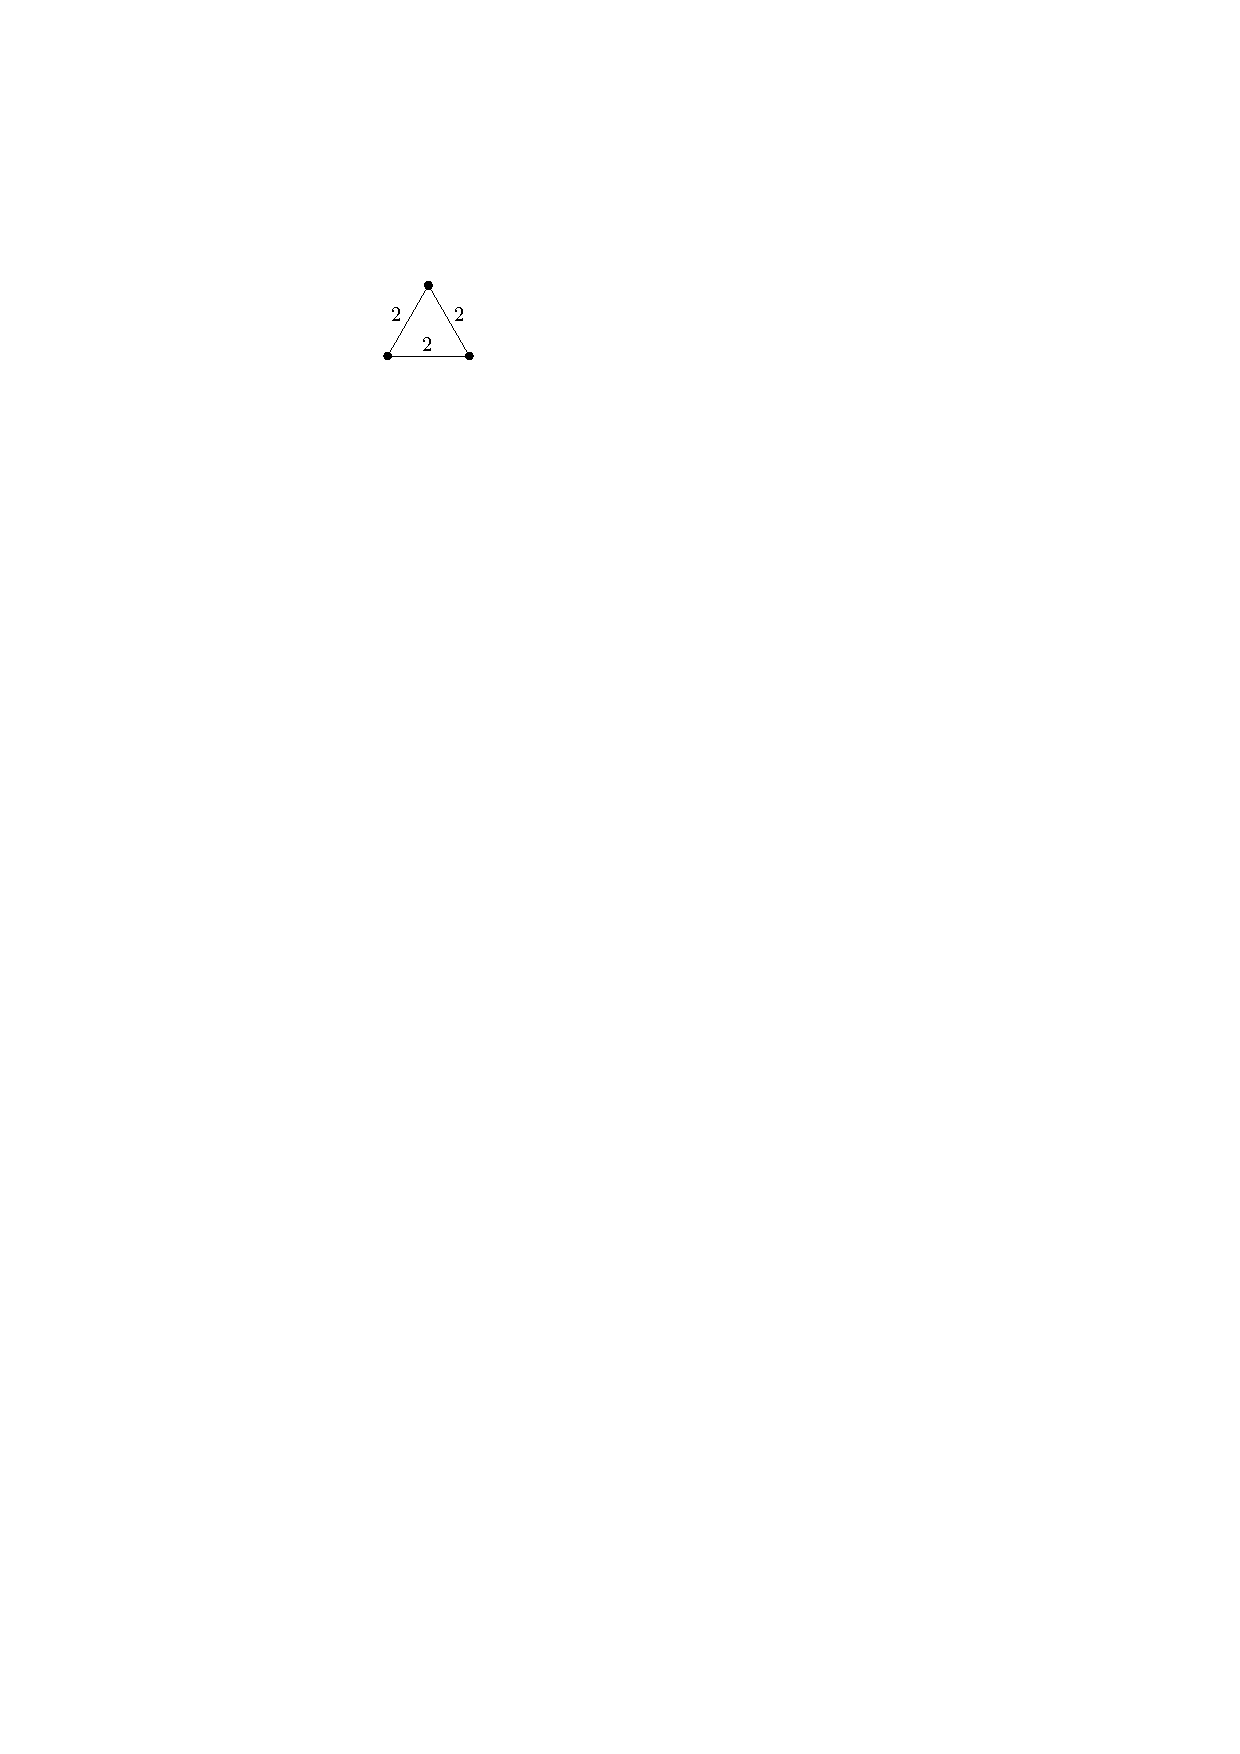
\includegraphics[scale=1]{img/example-act}
         \label{fig:example_act}
     \end{subfigure}
     \begin{subfigure}[t]{0.3\textwidth}
         \centering
         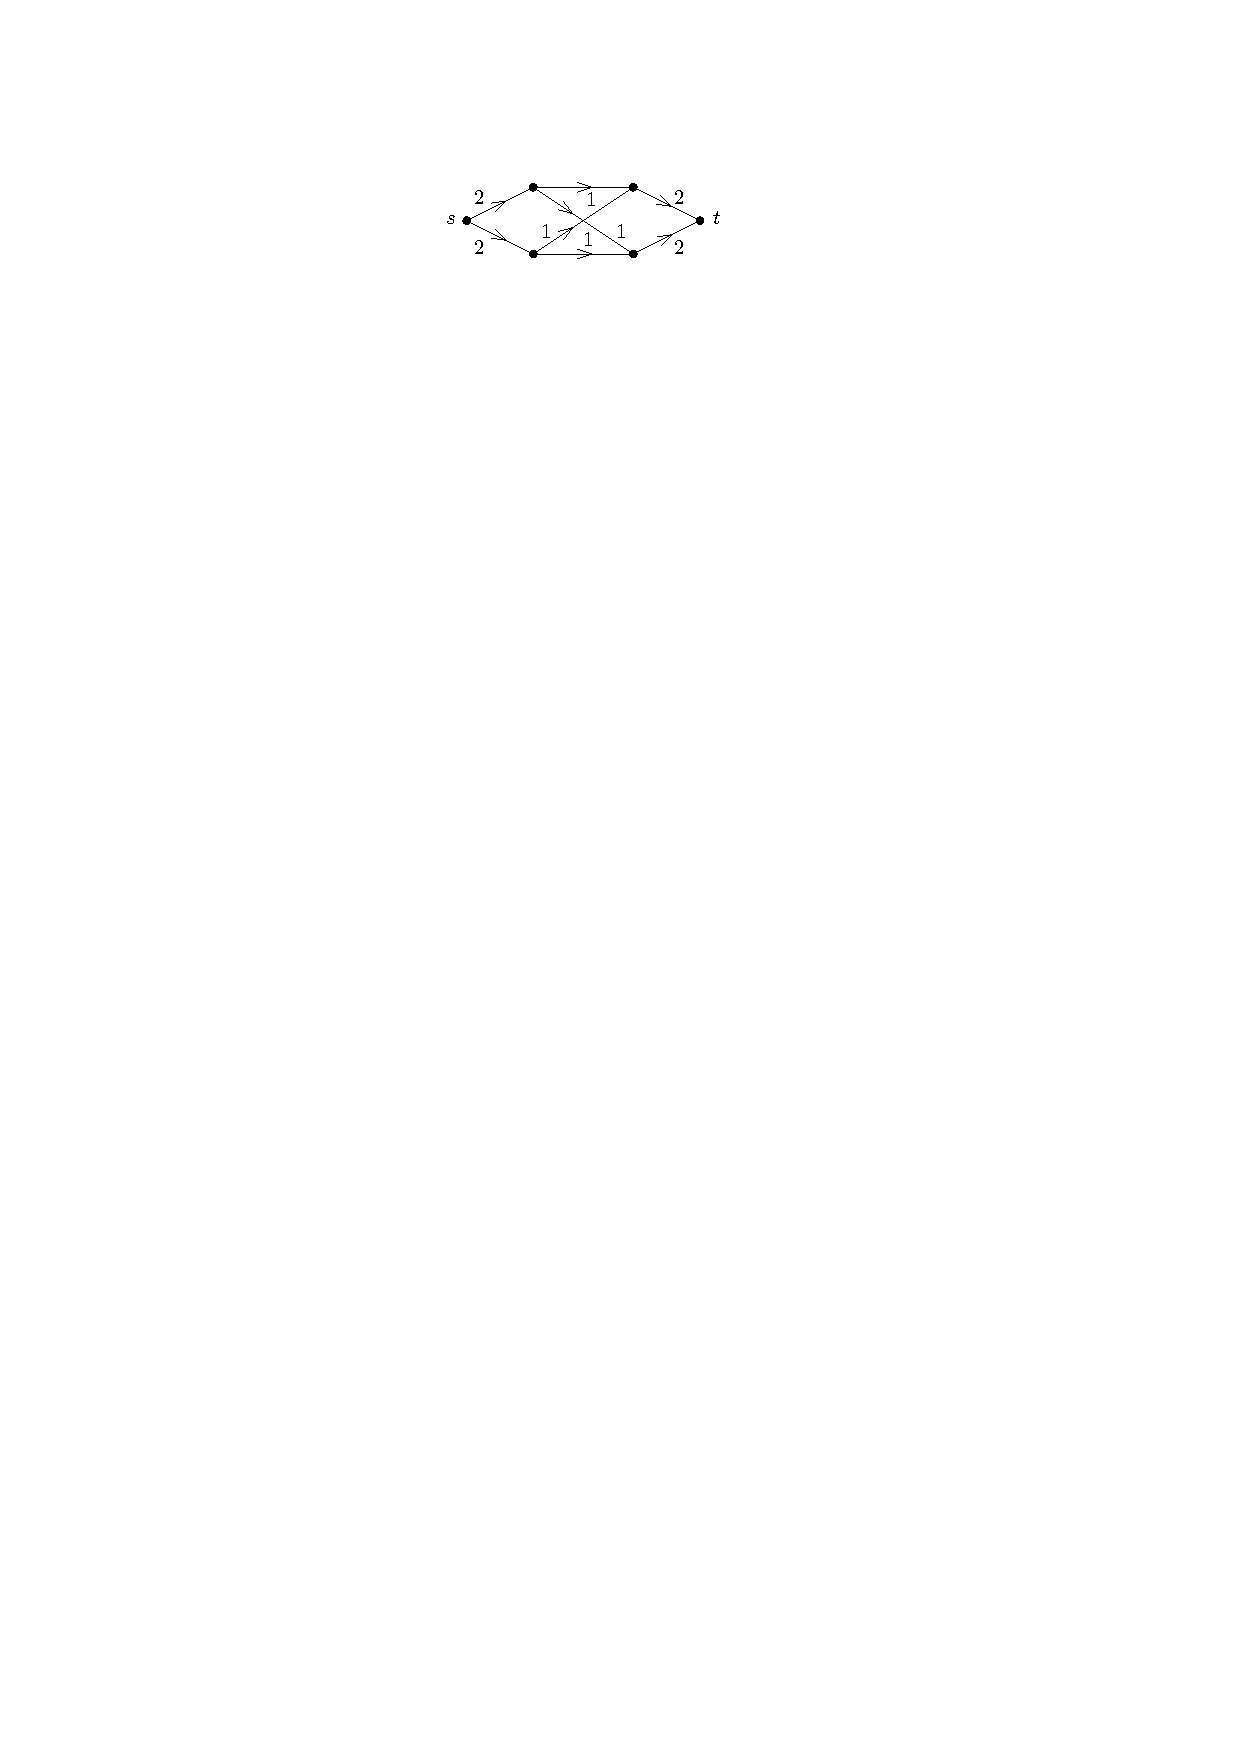
\includegraphics[scale=1]{img/example-st-act}
         \label{fig:example_st_act}
     \end{subfigure}
        \caption{Example instances for (a) problem \act\ and (b) problem \stact.}
        \label{fig:introduction_examples}
\end{figure}

We make use of the following graph-theoretic concepts and notations: Let $G = (V,E)$ be a directed or undirected graph. If $V' \subseteq V$ is a subset of the vertices, the corresponding \emph{edge cut} $\delta(V')$ is the set of edges having one endpoint in $V'$ and one endpoint in $V \setminus V'$ (in the directed case, we do not distinguish here between incoming and outgoing edges). For a vertex $v$, we let $\delta(v) := \delta(\set{v})$. If $(V_1,\dots,V_k)$ is a partition of $V$, the \emph{multicut} $\delta(V_1,\dots,V_k)$ is the set of edges with endpoints in diiferent parts of the partition. We denote by $G[V']$ the \emph{induced subgraph} on $V'$. By removing the vertex $v$ from $G$, we obtain $G - v := G[V \setminus \set{v}]$. Similarily, if $E' \subseteq E$ and $e \in E$, then $G - E' := (V, E \setminus E')$, and $G - e := G - \set{e}$. The \emph{treewidth} of a graph is an important parameter in the area of parameterized complexity (for an introduction, see e.g.\ [cite]).


\textbf{ Other Preliminaries: }
\begin{enumerate}
\item definition path (directed/undirected)
\item hamiltonian path/cycle
\item complete (bipartite) graph
\item $[n]$
\end{enumerate}

\section{NP-Hardness}
\label{sec:hardness}

In this section, we show NP-hardness of the problems \act\ and \stact, even if the input instances are restricted. This is done by reducing from the following two classical problems:

\vspace*{0.2cm}

Problem \textsc{Partition}: Given $A = \set{a_1, \ldots, a_n} \subseteq \N$, let $Q := 1/2 \sum A$. Does there exist $S \subseteq A$ with $\sum S = Q$?

\vspace*{0.2cm}

Problem \textsc{3-Partition} (variant): Given $A = \set{a_1, \ldots, a_{3n}}$ with $Q/4 < a_i < Q/2$ for all $i$, where $Q := 1/n \sum A$, does there exist a partition $A = A_1 \dotunion A_2 \ldots \dotunion A_n$ of $A$, such that $\sum A_j = Q$ for all $j$?

\vspace*{0.2cm}

It is known that \textsc{Partition} is NP-complete, but not strongly NP-complete, and that \textsc{3-Partition} is strongly NP-complete, meaning that there exists a polynomial $p$, such that \textsc{3-Partition} is NP-complete even if $a_i \leq p(n)$ for all $i$.

For each of the two problems $\act$ and $\stact$, we show hardness even if either the structure of the input, i.e.\ the treewidth is bounded by a constant, or if the lifetimes $w(e)$ are bounded by a constant. We start with the problem $\act$.

\subsection{Activation Problem}

\begin{theorem}
The problem \act\ is strongly NP-complete, even if the input graph is $K_{2,n}$.
\end{theorem}
\begin{proof}
Let $A = \fromto{a_1}{a_{3n}}$ be an instance of \textsc{3-Partition} and let $Q := 1/n \sum A$. Let $\beta := nQ + n - 1$. In order to prove NP-completeness, we construct an instance of problem \act\ whose optimal solution is $\beta$, if and only if $A$ is a yes-instance of \textsc{3-Partition}. Consider the  complete bipartite graph $K_{2,4n-1}$ on the two vertex sets $\set{s, t}$ and $\set{x_1, \ldots, x_{n-1}, y_1, \ldots, y_{3n}}$. For $i \in [n-1]$, we let $w(\set{s,x_i}) := i(Q + 1)$ and $w(\set{x_i,t}) := (n - i)(Q + 1)$. For $i \in [3n]$, we let $w(\set{s,y_i}) := a_i$ and $w(\set{y_i,t}) := \beta$. 

Now, assume that for the described instance, there exists a schedule $\sigma$ of value $\beta$. Note that for all $i \in [n-1]$, we have $w(\set{s,x_i}) + w(\set{x_i,t}) = \beta + 1$, hence the sum of all weights is $(n-1)(\beta + 1) + 3n\beta + (\beta - n + 1) = \beta 4n$. Because the set of active edges is spanning at each point in time, and a spanning tree of $K_{2, 4n-1}$ has $4n$ edges, this implies that all of the graphs $G_1, \dots G_\beta$ have exactly $4n$ edges and are spanning trees. For $i \in [n-1
]$, consider vertex $x_i$.  Due to $w(\set{s,x_i}) + w(\set{x_i,t}) = \beta + 1$, there is exactly one $k \in [\beta]$, such that $d_k(x_i) = 2$. Furthermore, because the scheduling of the edges is nonpreemptive, and clearly $d_1(x_i) \geq 1$ and $d_\beta(x_i) \geq 1$, we can further deduce that $k$ has only the two possible values $i(Q+1)$ or $(n-i)(Q+1)$. Additionally, if there exists a $k$ such that for distinct $i, i' \in [n-1]$ one has $d_k(x_i) = d_k(x_{i'}) = 2$, then $G_k$ has a cycle, which is impossible. We conclude that there exists some $i \in [n-1]$ with $d_k(x_i) = 2$ if and only if $k \in \set{Q+1, 2(Q+1), \dots (n-1)(Q+1)}$. But this is a set of $n-1$ equidistant numbers, in $[\beta]$, such that $n$ gaps of size $Q$ are created. Using again acyclicity of $G_1, \dots, G_\beta$, it is then easy to see that the scheduling of the edges $\fromto{\set{s,y_1}}{\set{s,y_{3n}}}$ implies a correct 3-partion of $A$.

%Note that $w(sx_i) + w(x_it) = nQ + n + 1$. Hence it is easy to see, that a schedule of value $nQ + n + 1$ does not exist. We claim that a schedule of length $nQ + n$ exists, if and only if $A$ can be 3-partitioned. Suppose such a schedule $\sigma$ exists. Then for each $i \in [n]$, there is some $t_i$ such that $T(sx_i) \cap T(x_it) = [t_i, t_i + 1]$. Because $\val(\sigma) = nQ + n$, we have $t_i \neq t_j$ for $i \neq j$, so w.l.o.g., we have $t_i = iQ + i - 1$. Up so far, this means that $s$ and $t$ are connected during $[t_1, t_1 +1]$, $[t_2, t_2 + 1], \ldots [t_n, t_n + 1]$. Hence the scheduling of the edges $\fromto{y_1t}{y_{3n}t}$ needs to fill the \enquote{gaps} of size $Q$ between these intervals and therefore implies a 3-partition of $A$.

On the other hand, assume $A$ is a yes-instance. Then it is easy to see that a schedule of value $\beta$ exists. (The schedule has the same properties as the schedule $\sigma$ in the first direction of the proof.)
\end{proof}

%We wish to show that, analogoulsy, \act\ is NP-complete, even if the lifetimes are bounded by a constant. However, it is not clear whether a gadget similar to the one used in \cref{lemma_gadget} exists. The difficulty is that each time that we introduce a new vertex $v$, in a valid schedule $v$ must be connected by active edges to the rest of the graph at all times. Instead, we use a diiferent approach.
This shows hardness, even if the treewidth of the input is bounded by two. We now show hardness even if the lifetimes $w(e)$ are bounded. For this, we reduce from the Hamilton cycle problem. Akiyama, Nishizeki and Saito proved that the Hamilton cycle problem is NP-complete even for bipartite, 3-regular graphs \cite{hamilton3regularBip}. We additionally require hardness for a more restricted variant of the hamilton cycle problem, which we call \textsc{Hamilton'}. The following lemma is surely known, however, we were unable to find it in the literature. We give a proof of this lemma in 

\begin{lemma}
\label{hamilton_cycle_lemma}
The Hamilton cycle problem for a graph $H$ is NP-complete, even under the following restrictions: The graph $H$ is undirected, bipartite, and 4-regular. Furthermore, as part of the input we are given a special edge $\set{u, z}$, such that $H$ has a Hamilton cycle iff $H$ has a Hamilton cycle using the edge $\set{u, z}$ iff $H$ has a Hamilton path starting at $u$.
\end{lemma} 

\begin{proof}
Fix some vertex $w \in V$. Let $G_1$, $G_2$ be two copies of $G$. For each $v \in V \setminus \set{w}$, take a copy $X_v$ of $K_{4,4}$, remove some edge $u_1u_2$ from $X_v$, and add edges $v_1u_1$ and $u_2v_2$, where $v_i$ is the copy of $v$ in $G_i$, $i = 1,2$. Finally take two copies $X_w$ and $X'_w$ of $K_{4,4}$, remove an edge ${u_1u_2}$ from $X_w$ and an edge $u'_1u'_2$ from $X'_w$, add edges $w_1u_1$, $u_2u'_1$, $u'_2w_2$ and set $x := u_2$, $y := u'_1$ where $w_i$ is the copy of $w$ in $G_i$. It is not hard to see that this graph has the claimed properties.
\end{proof}

\begin{lemma}
Let $G'$ be a 3-regular, bipartite graph. There exist a graph $G = (V,E)$ and a map $l: E \rightarrow \fromto{1}{6}$, both computable in polynomial time, such that $(G, l)$ has a schedule of value 7 for the activation problem, if and only if $G'$ has a Hamiltonian cycle. 
\end{lemma}
\begin{proof}
First, construct $H, x$ and $y$ from $G'$ like in \cref{hamilton_cycle_lemma}.  We claim that the graph $G = (V, E)$ from \cref{fig_act_hamilton_cycle} (a) has the desired property. Let $H$ be bipartite on the two parts $U = \fromto{u_k}{u_k}$ and $W = \fromto{w_1}{w_k}$ such that $x = u_k$ and $y := w_k$. Let $e_0 := xy$. Then $G$ consists of a copy of $H$ where every edge has lifetime 2, except $e_0$, which has lifetime 1. Furthermore, there is an additional vertex $x$, which is connected to each of $\fromto{u_1}{u_k}$ via the gadget $L$ and to each of $\fromto{w_1}{w_k}$ via the gadget $R$. Finally, there is an additional vertex $y$ connected to both $x$ and $y$ with an edge of weight 4.

For a schedule $\sigma$ of value 7, let for $t \in \fromto{1}{7}$, $G_t := (V, A(t-1/2))$ be like in \cref{sec_notation}. We first describe the properties of the gadgets $L$ and $R$: Note that the sum of all lifetimes in $G$ is $8k - 1 + 39k + 16k + 8 = 63k + 7 = 7(|V(G) - 1|)$. Therefore, each of $G_{1}, \ldots, G_{7}$ is a tree, and in particular acyclic. By inspecting the vertices $r_1$ and $r_2$ and using acyclity of $G_2, G_6$ we see that the gadget $R$ necessarily connects $x$ and $w_i$ in $G_2$ and $G_6$ and does not connect $x$ and $w_i$ in $G_t$ for $t \neq 2,6$. Similarily, the gadget $L$ necessarily connects $x$ and $u_i$ in $G_3$ and $G_5$ and has some remaining edges, which are not restricted and behave like two parallel edges of lifetime 1. Analogously, $G_{t}[\set{x, y, w_k}]$ is connected if and only if $t = 4$.

Now, suppose $G'$ has a Hamiltonian cycle. By \cref{hamilton_cycle_lemma}, there exists a Hamiltonian cycle $C$ in $H$, which uses $e_0$. Then $H - E(C)$ is 2-regular, hence there exist disjoint matchings $M_1, \ldots, M_4$ such that $M_1 \dotunion M_2 = E(C)$ and $M_3 \dotunion M_4 = E(H) \setminus E(C)$ and $e_0 \in M_1$. Then we schedule $e_0$ in $G_3$; $M_1 \setminus \set{e_0}$ in $G_3, G_4$; $M_2$ in $G_4, G_5$; $M_3$ in $G_1, G_2$; and $M_4$ in $G_6, G_7$. We schedule the gadgets such that $U$ is connected to $x$ via the $L$'s in $G_1, G_3, G_5$ and $ G_7$, and that $W$ is connected to $x$ via $R$'s in $G_2$ and $G_6$, and that $x$ is connected to $w_k$ via $y$ in $G_4$. Now observe that the active edges in $U \cup W$ form a matching of $H$ in $G_1, G_2, G_3, G_5, G_6$ and $G_7$ and a Hamiltonian path in $G_4$. It is easy to see that this is a valid schedule of value 7. 

On the other hand, suppose there exists a schedule $\sigma$ of value 7 for $(G, l)$.
  
Recall the properties of the gadgets $L$ and $R$. Then, for $t' \in \set{1, 7}$, consider $G_{t'}$ and some $w_i$ for $i \in \fromto{1}{k-1}$. Note that for all $t \in \set{1, 3, 4, 5, 7}$ at least one of the edges in $\delta(w_i) \cap E(H)$ is active. This implies that $w_i$ has degree 1 in $G_{t'}[U \cup W]$, due to the different possibilities of covering the set $[0, 1] \cup [2, 5] \cup [6, 7]$ with 4 intervals of length 2. Similarly, by considering $t \in \set{1, 3, 5, 7}$, we see that $w_k$ has degree 1 in $G_{t'}[U \cup W]$ and that $e_0 \not \in E(G_{4})$. So all $w \in W$ have degree 1 in $G_{t'}[U \cup H]$. But this implies that $G_{t'}[L']$ is connected for each copy $L'$ of $L$, otherwise $U$ is disonnected in $G_{t'}$. Hence $G_t[L']$ is connected if and only if $t \in \set{1, 3, 5, 7}$. Hence, for $u \in U$ and $t' \in \set{2, 6}$, we have that the degree of $u$ in $G_{t'}[U \cup W]$ is at least one. Finally, consider $F := G_{4}[U \cup W]$: Due to the restrictions of the minimum degrees for $t' \in \set{1, 7}$ or $t' \in \set{2, 6}$, we have that the maximum degree in $F$ is two. Similarly as before, we see that the degree of $u_k$ in $F$ is 1. Note that $F$ is connected. We conclude that $F$ is a Hamiltonian path in $H$ starting at $u_k$. By \cref{hamilton_cycle_lemma}, $G'$ has a Hamiltonian cycle.

%%Due to the different possibilities of covering the interval $[0, 7]$ with four intervals of length 2, we have that for $t' \in \set{0.5, 6.5}$, each of $w_1, \ldots w_{k-1}$ has degree 1 in $G_{t'}$. Similarly, both $y, w_k$ have degree 1 in $G_{t'}$. We conclude that $u_1, \ldots, u_k$ lie in $k$ different connected components of $G_{t'} - x$ and hence $G_{t'}$ has an edge connecting $x$ and $u_i$ for each $i$. But then, $G_{3.5}$ has none of the edges between $x$ and $u_i$, hence $G_{3.5}[Z]$ is connected, where $Z := \set{u_1, \ldots, u_k, w_1, \ldots, w_k}$.  Again, by the different possibilities of covering the interval $[0, 7]$ with subintervals, we conclude that in $G_{3.5}$, the vertices $u_k, w_k$ have degree 1, $e_0 \not\in E(G_{3.5})$, and each of $w_1, \ldots w_{k-1}$ have degree at most two. They also have degree exactly two, otherwise we find a cyle in one of $\set{G_{0.5}, \ldots, G_{6.5}} \setminus \set{G_{3.5}}$. 
\end{proof}
\begin{figure}[htpb]
\centering
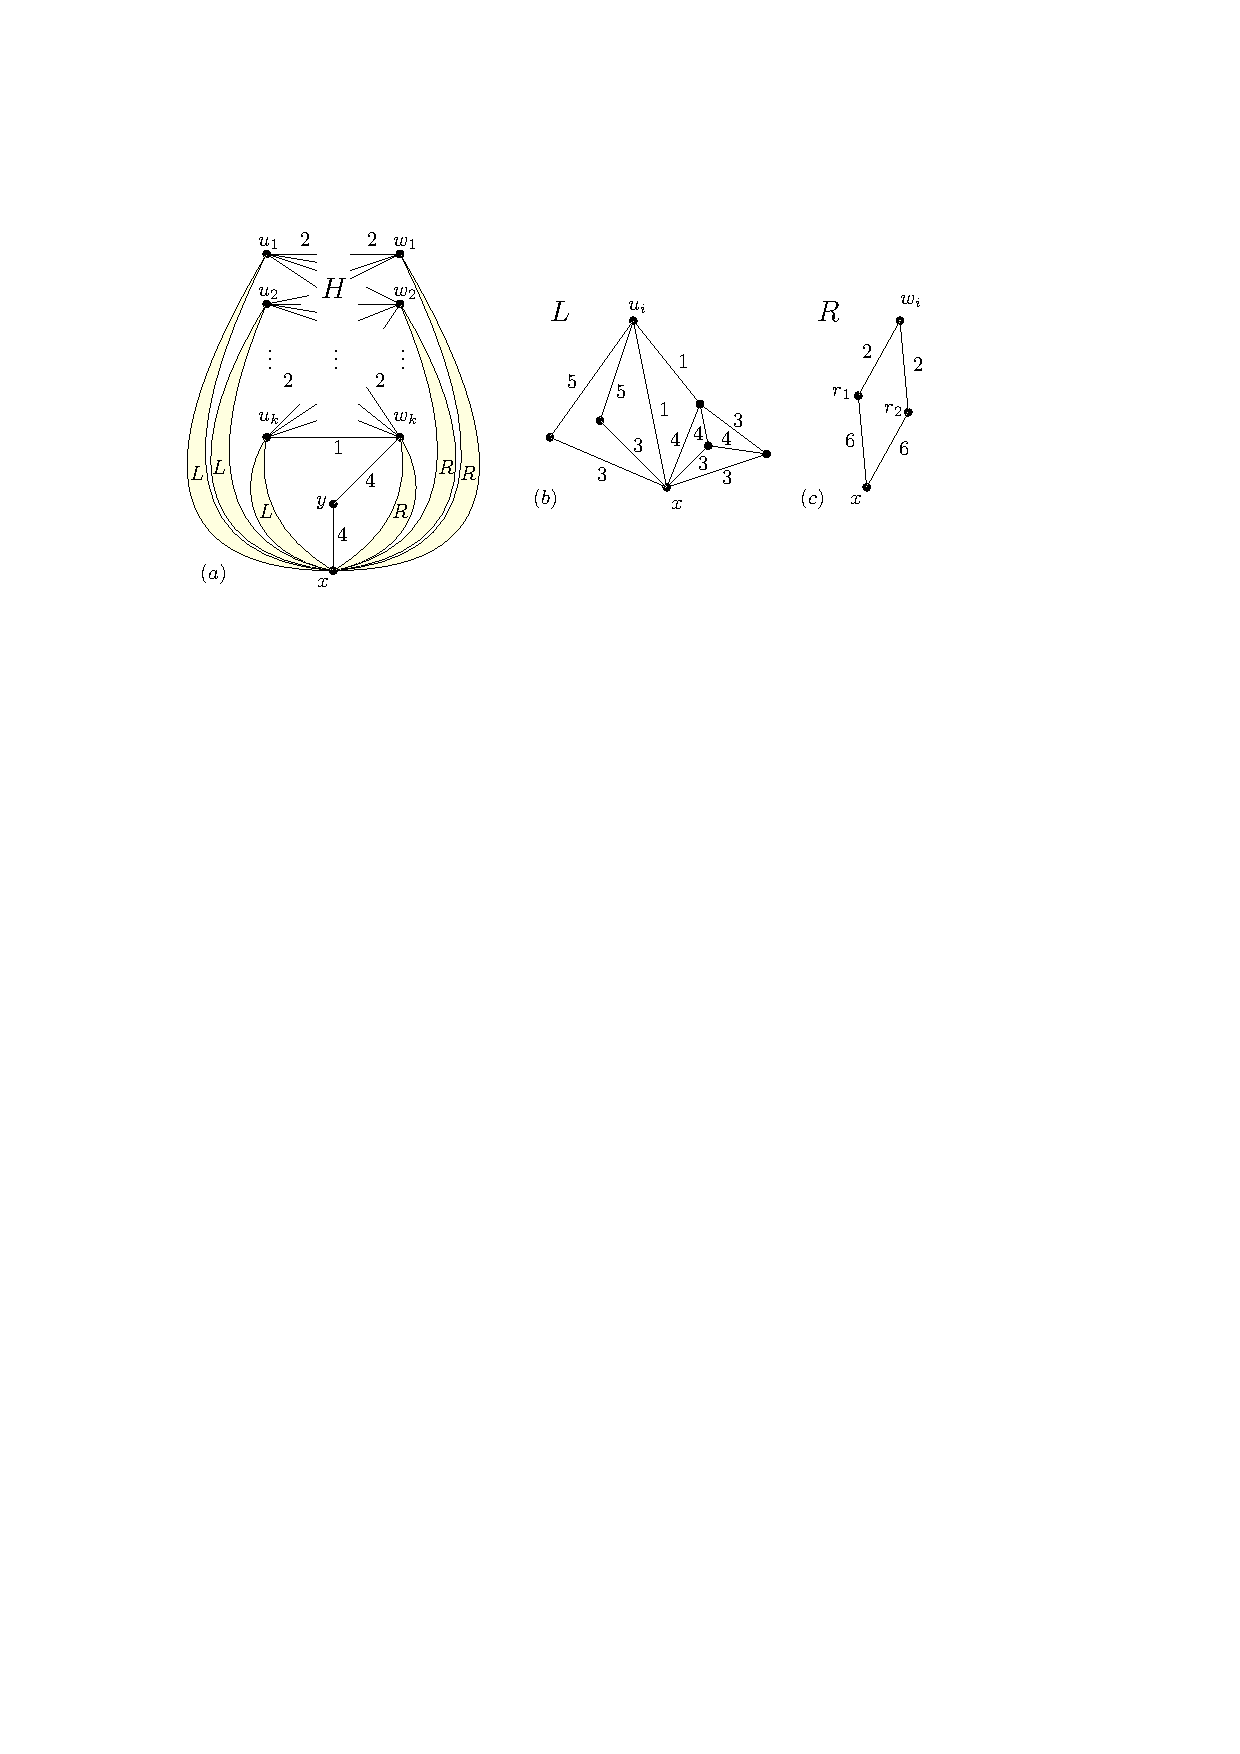
\includegraphics[scale=1]{img/act-hamilton-cycle}
\caption{(a) Reduction \textsc{Hamilton'} $\rightarrow$ \act. (b) The gadget $L$. (c) The gadget $R$.}
\label{fig_act_hamilton_cycle}
\end{figure}

\begin{corollary}
The problem \act\ is NP-complete, even if $l(e) \in \fromto{1}{6}$ for all edges.
\end{corollary}

\begin{corollary}
\label{corollary_act_no_approx}
If $P \neq NP$, then the problem \act\ can not be approximated in polynomial time by a factor better than 7/6, even if $l(e) \in \fromto{1}{6}$ for all edges. 
\end{corollary}

\subsection{$s$-$t$-Activation Problem}
We now show hardness of the problem $\stact$, even if either the structure (i.e.\ the trewidth) or the lifetimes of the input are bounded by a constant. We begin with the case of bounded structure.

\begin{theorem}
\label{thm_stact_np_hard}
The problem \stact\ is NP-complete, even if the input graph is planar with treewidth at most 3.
\end{theorem}

\begin{proof}
Let $(A = \fromto{a_1}{a_n}, Q)$ be an instance of \textsc{Partition}, consider the graph from \cref{fig_stact_np_hard}. We claim that there exists a schedule of value $4Q$ if and only if $A$ can be partitioned. Suppose $\sigma$ is such a schedule. By symmetry we can assume $\sigma(sv_1) = \sigma(v_1w_1) = 0$. Then also $\sigma(v_1w_2) = Q$, otherwise we are inefficient and can not reach $4Q$ anymore. Then by a similar reasoning concerning efficiency, the scheduling of the edges between $w_1$ and $t$ implies a partition of $A$ into two equal parts. The other direction of the claim is easy to see. Finally, note that the involved graph is planar and has treewidth 3.
\end{proof}
\begin{figure}[htpb]
\centering
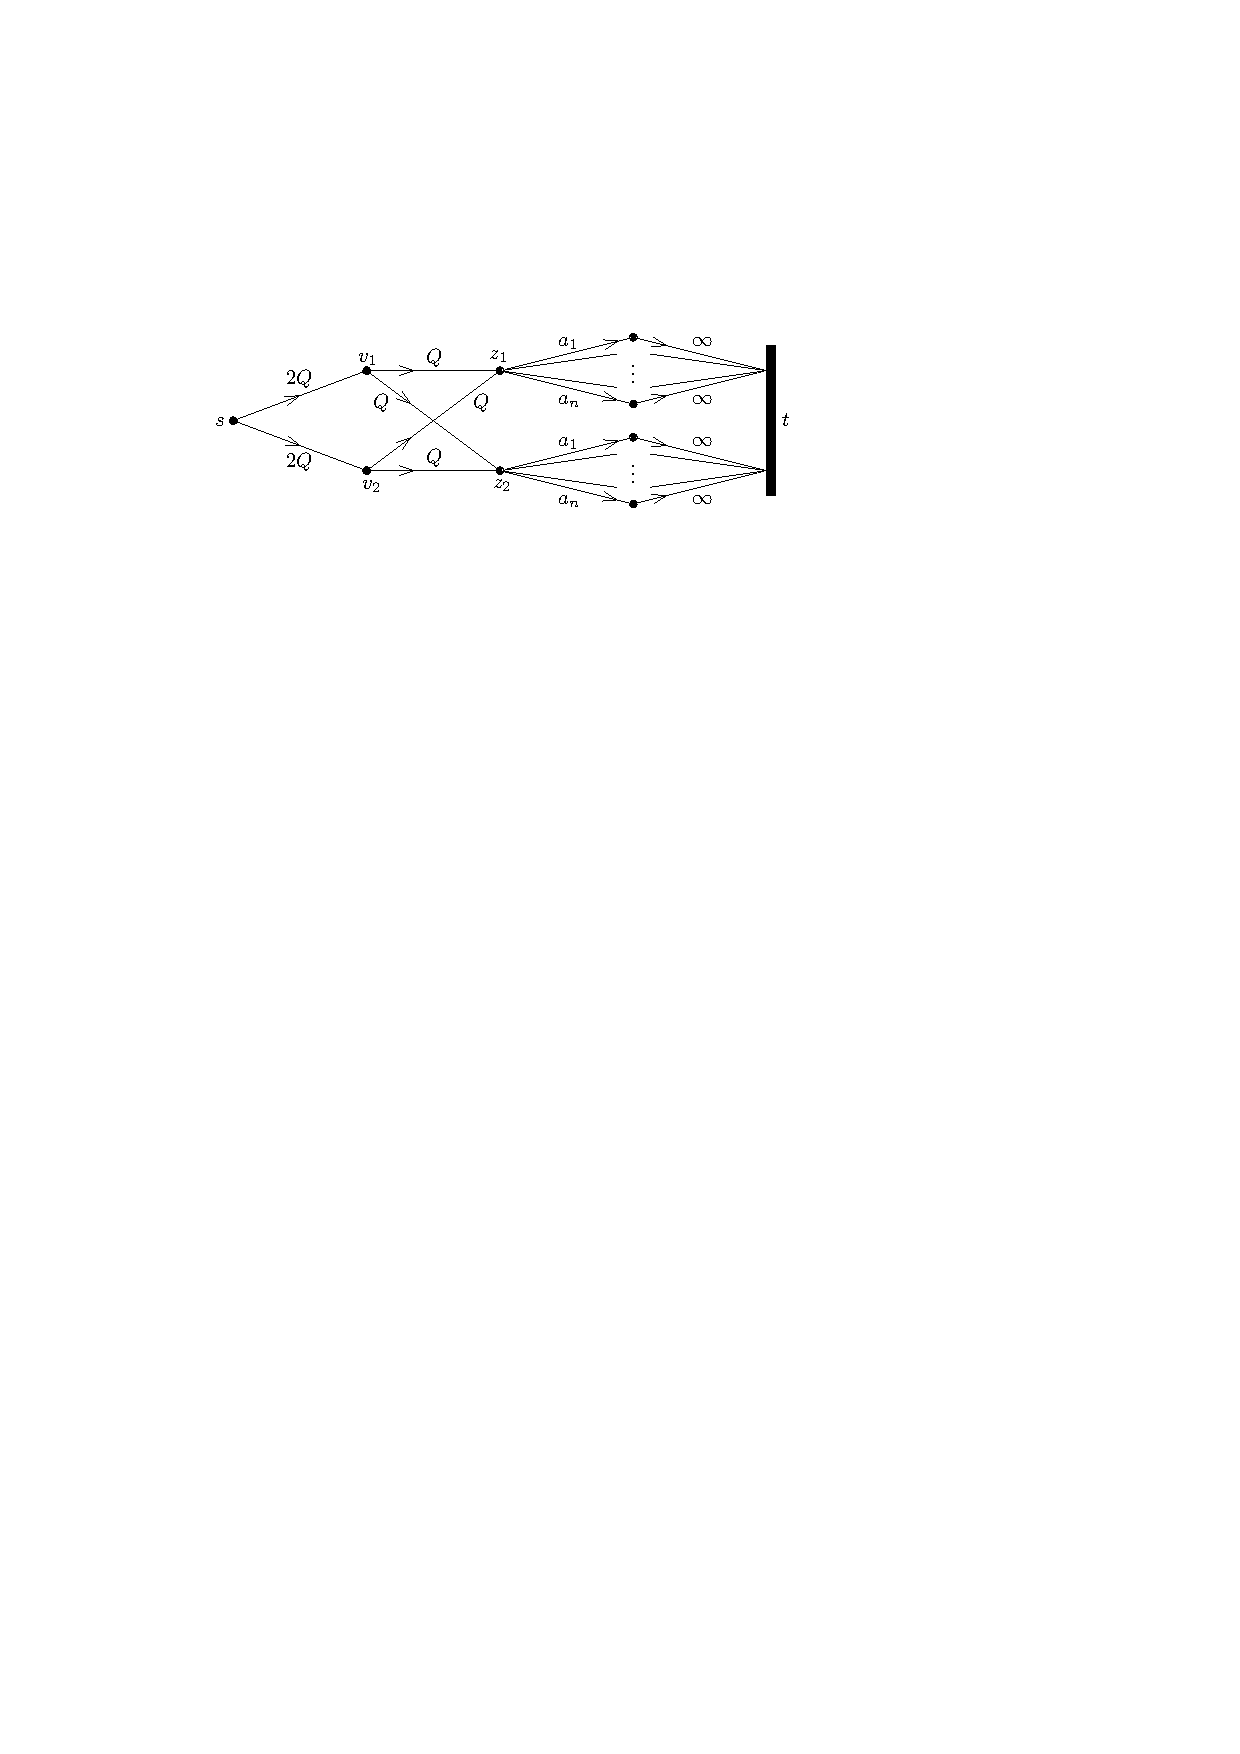
\includegraphics[scale=1]{img/st-act-np-hard}
\caption{Reduction \textsc{Partition} $\rightarrow$ \stact\ described in \cref{thm_stact_np_hard}.}
\label{fig_stact_np_hard}
\end{figure}

We wish to prove that \stact\ is NP-complete, even if the lifetimes are restricted to $\set{1, 2}$. For this, we first prove the following weaker lemma, whose proof utilizes the same idea as the previous proof:

\begin{lemma}
\label{lemma_st_act_strongly_np_hard}
The problem \stact\ is strongly NP-complete. 
\end{lemma}
\begin{proof}
Let $(A = \fromto{a_1}{a_{3n}}, Q)$ be an instance of \textsc{3-Partition}. Consider the graph sketched in \cref{fig_stact_strongly_np_hard}. Here, there is an edge of lifetime $nQ$ between $s$ and $v_i$ for all $i$, there is a complete bipartite graph between $\fromto{v_1}{v_n}$ and $\fromto{w_1}{w_n}$ with every edge having lifetime $Q$, and the symbol $A$ represents $3n$ parallel edges with lifetimes $a_1, \ldots, a_{3n}$. We claim there is a schedule of value $n^2Q$, if and only if $A$ can be 3-partitioned. If $\sigma$ is such a schedule, we can assume by ($n$-fold) symmetry, that $\sigma(sv_i) = (i - 1)nQ$ for all $i \in [n]$. Let for $i \in [n]$, $P_i := [(i-1)nQ, inQ]$ denote the $i$-th phase of $\sigma$. During $P_i$, the edges $\fromto{v_iw_1}{v_iw_n}$ get activated in some order, let $v_iw_{f(i)}$ be the last edge in this order. Call a vertex $w_j$ exceptional, if $w_j = w_{f(i)}$ for some $i \in \fromto{1}{n-1}$. At least one vertex $w'$ is not exceptional, and the scheduling of the edges between $w'$ and $t$ implies a 3-partition of $A$. The other direction of the claim is easy to see.
\end{proof}
\begin{figure}[htpb]
\centering
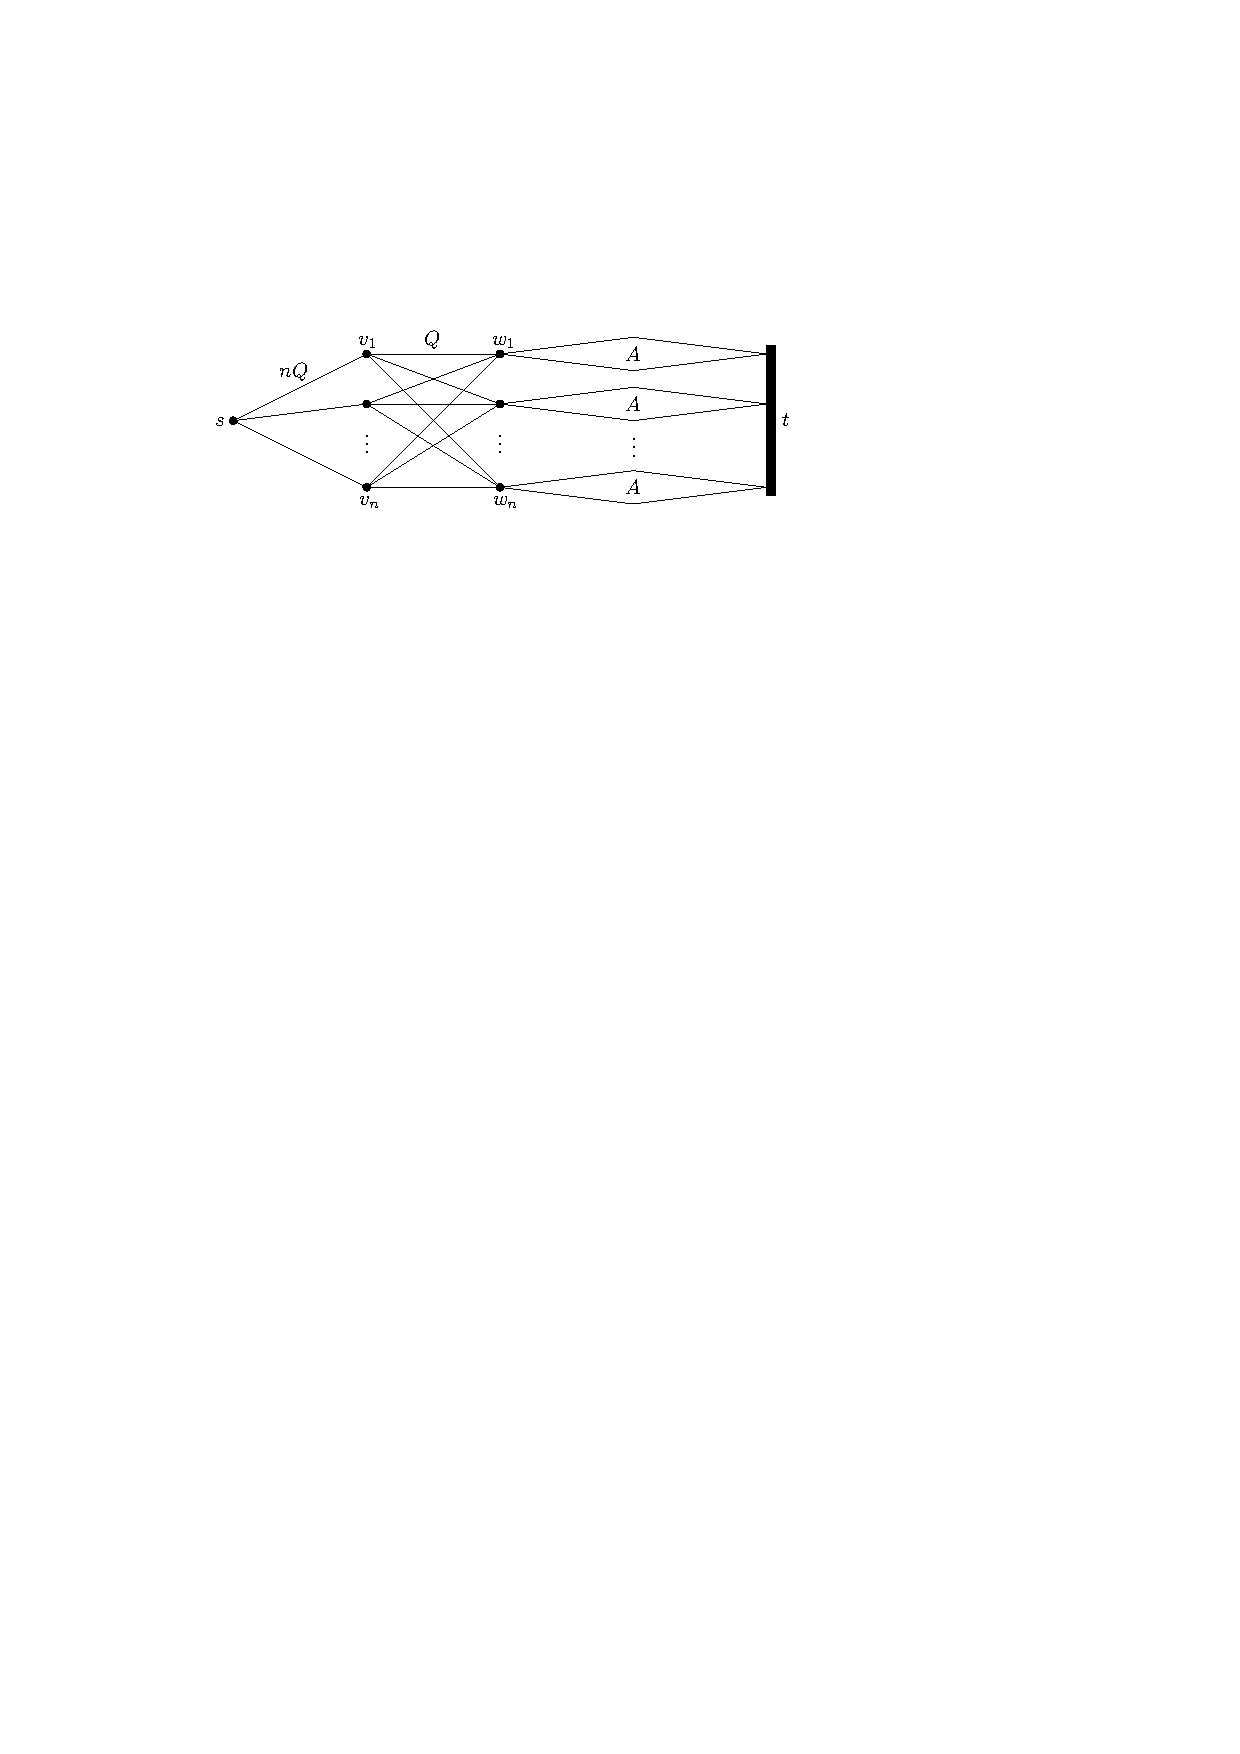
\includegraphics[scale=1]{img/st-act-strongly-np-hard}
\caption{Reduction \textsc{3-Partition} $\rightarrow$ \stact\ described in \cref{lemma_st_act_strongly_np_hard}.}
\label{fig_stact_strongly_np_hard}
\end{figure}

We introduce a gadget graph $G_k$, whose edges have lifetimes restricted to $\set{1,2}$, such that $G_k$ behaves quite similar to a single edge of lifetime $2k - 1$.

\begin{lemma}
\label{lemma_gadget}
Let $G_k$ be the graph depicted in \cref{fig_gadget}. Let $\sigma$ be some (not necessarily valid) schedule for $G_k$ and let $C(\sigma)$ be like in \cref{sec_notation}. Then we have that \begin{enumerate}[(i)]
\item $|C(\sigma)| \leq 2k -1$,
\item $|C(\sigma)| = 2k -1$ can be achieved for some $\sigma$, and
\item If $|C(\sigma)| = 2k -1$, then $C(\sigma)$ is an interval in $\N_0$. \label{lemma_gadget_case_3}
\end{enumerate}
\end{lemma}
\begin{proof}
Claims (i) and (ii) are easy to see. For claim (iii), assume the contrary, i.e.\ $|C(\sigma)| = 2k -1$ and $C(\sigma) = I_1 \cup \dots \cup I_m$ where $m \geq 2$ and $I_j = \fromto{a_j}{b_j}$ and $a_{j+1} > b_j + 1$ for all $j < m$. Then at least one of the intervals, say $I_1$, has an odd cardinality. Notice that the set of edges contributing to $I_1$ (i.e.\ the set $E_1 := \set{e \in E(G_k) : \sigma(e) \leq b_1}$) is disjoint from the set of edges contributing to $I_2$ (i.e.\ the set $E_2 := \set{e \in E(G_k) : \sigma(e) + l(e) > a_2}$). Consider the cuts $\delta(s)$ and $\delta(t)$, both of which have capacity $2k$. Because $|I_1|$ is odd, but the edges in $\delta(s)$ and $\delta(t)$ have lifetime 2, at least one unit of capacity from both $\delta(s)$ and $\delta(t)$ is wasted in $E_1$. Now, applying a similar argument like in claim (i) to $E_2$ and $I_2$ yields $|C(\sigma)| < 2k - 1$, a contradiction. 
%and $C(\sigma)$ is not an interval. Let $t_0 := \min C(\sigma)$. Because at most one unit of time from each of the cuts $\delta(s)$ or $\delta(t)$ is \enquote{wasted}, but at time $t_0 + 1$ a unit either in $\delta(s)$ or $\delta(t)$ is wasted, we have $t_0 + 1 \not\in C(\sigma)$. But then at time $t_0 + 2$ the situation looks isomorphic to \cref{fig_gadget} (b) and together with $v_1w_2$ and $v_kw_1$ we have already wasted 4 units of time. However, if we want to achieve a value of $2k - 1$ we can at most waste 3 units.
\end{proof}
\begin{figure}[htpb]
\centering
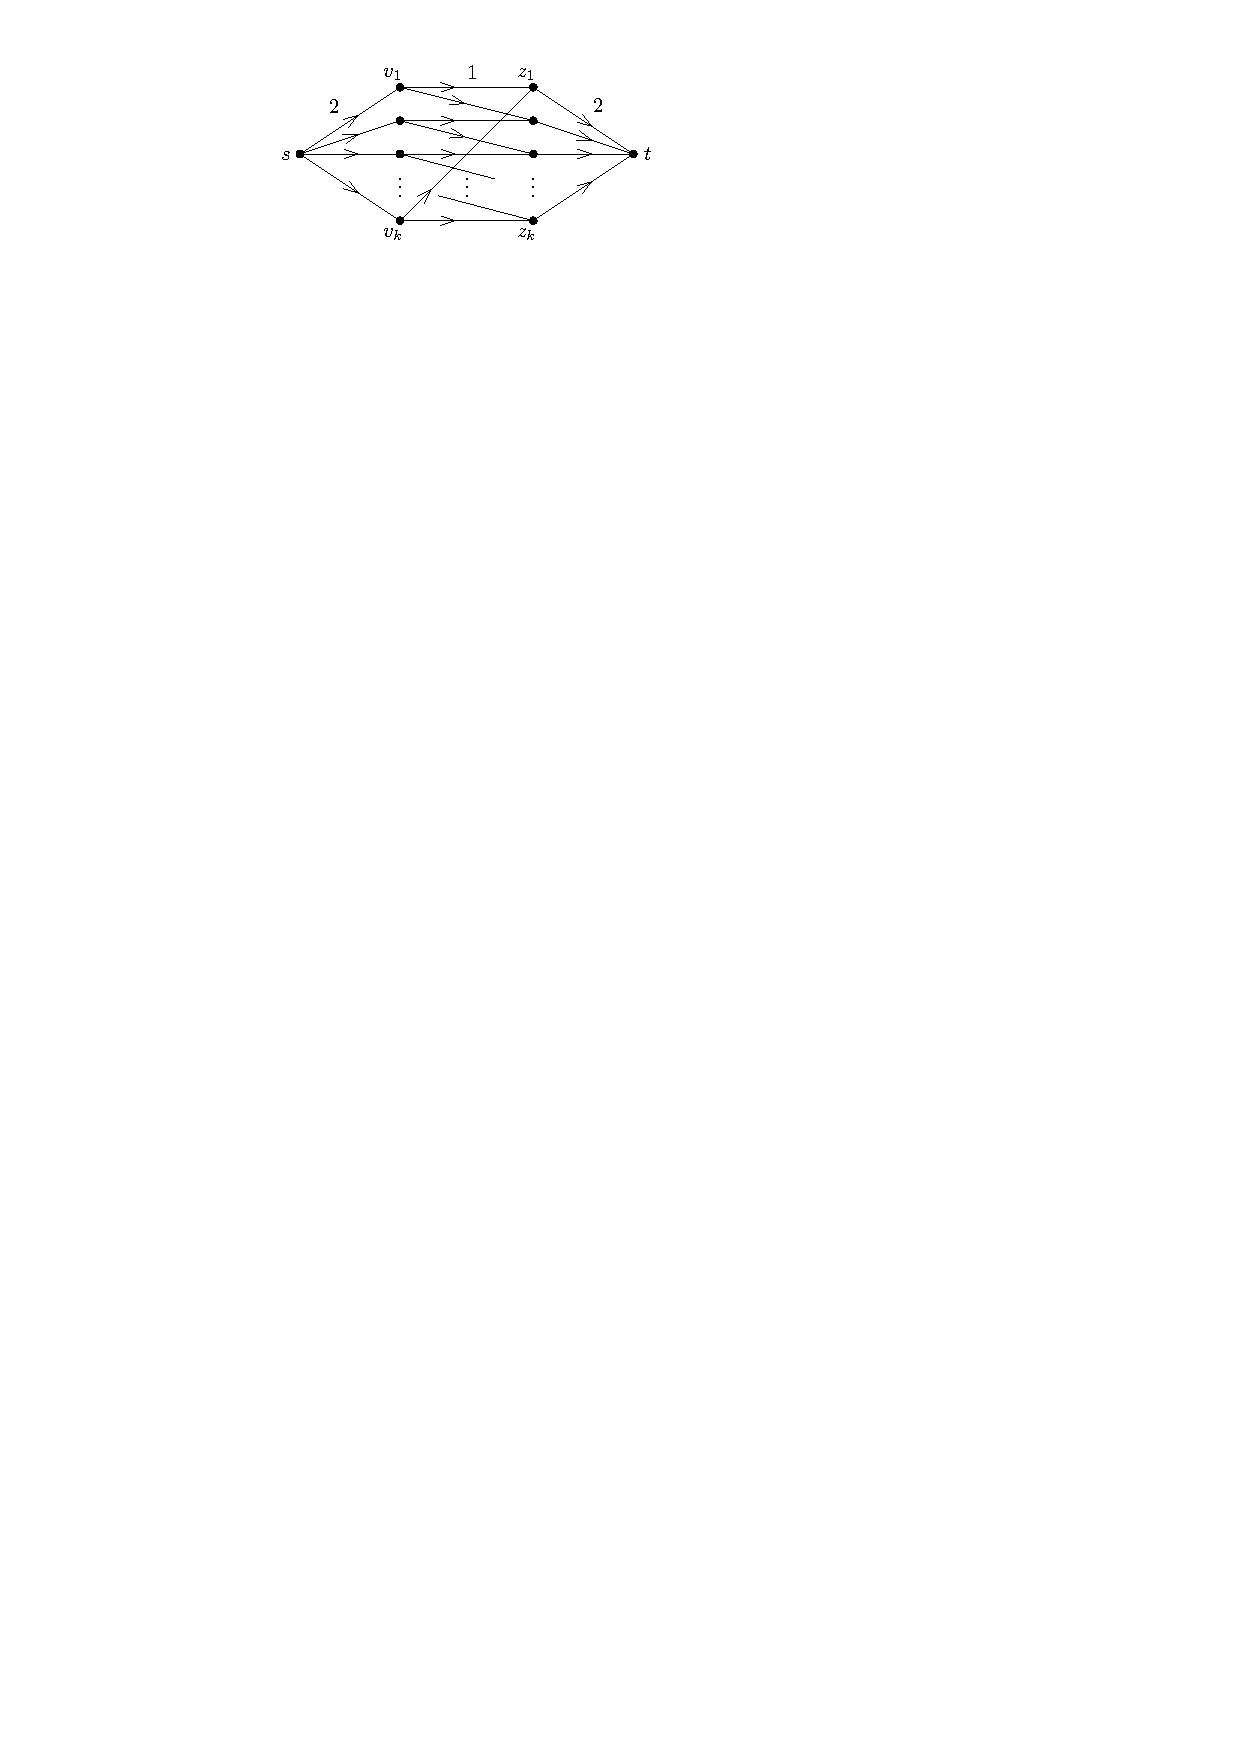
\includegraphics[scale=1]{img/gadget-new}
\caption{Gadget graph $G_k$.}
\label{fig_gadget}
\end{figure}

\begin{theorem}
The problem \stact\ is NP-complete, even if $l(e) \in \set{1, 2}$ for all edges.
\end{theorem}
\begin{proof}
Reduction from \textsc{3-Partition}. Let $(A = \fromto{a_1}{a_{3n}}, Q)$ be an instance of \textsc{3-Partition}, such that $a_i \leq p(n)$ for a suitable polynomial $p$. We can assume that $n$ is odd (otherwise, let $a_{3n+1} = a_{3n + 2} := 1$ and $a_{3n + 3} :=  Q - 2$) and each $a_i$ is odd (otherwise, let $a_i' := 2a_i + 1$). Then $Q$ is odd. Now, consider the same reduction as in \cref{lemma_st_act_strongly_np_hard}, where we substitute an edge of length $2k - 1$ by the gadget $G_k$. If a schedule of value $n^2Q$ exists, we need to use each gadget to its full extent, and \cref{lemma_gadget} (iii) is applicable. The rest of the proof is analogous to \cref{lemma_st_act_strongly_np_hard}.
\end{proof}


\section{Positive Results}
\label{sec:positive_results}

Consider a graph $G$ with treewidth bounded by a constant $k$ and edge weights bounded by a  constant $L$. As stated in the introduction, we exclude parallel edges. Then in particular there is a vertex of degree at most $k$ in $G$, therefore the size of a solution to \act, i.e.\ the value of a valid schedule, is at most $kL =: T$. (This is not true anymore in the presence of parallel edges.) We prove:

\begin{theorem} \label{thm_dynamic_program}
Let $k, T \in \N$. Let $(G, l)$ be an instance of \act, such that $G$ has treewidth at most $k$ and the size of an optimal solution is at most $T$. Then an optimal soultion can be computed in time $\bigO(T^{k^2}B(k+1)^{2T}n)$ (where $B(k+1)$ is the $(k+1)$-st Bell number).
\end{theorem}

\begin{corollary}
If both treewidth and maximum lifetime is bounded by $k$, the problem \act\ can be solved in time $(k+1)^{\bigO(k^3)}n$.
\end{corollary}

\begin{proof}[Proof of \cref{thm_dynamic_program}]
Let $n := |V(G)|$. Let $\mathcal{T} = (T, \set{X_t}_{t \in V(T)})$ be a (rooted) nice tree decomposition of $G$ of width at most $k$, where w.l.o.g.\ $V(T) = \set{1, \ldots, z}$ for some $z = \bigO(kn)$. For a bag $X_i$, let $V_i$ be the union of the vertices in $X_i$ and the vertices in the bags $X_j$ corresponding to all descendents $j$ of $i$ in $T$. (The vertex $j$ is a descendent of $i$, if it has a bigger distance to the root than $i$.)

For a bag $X_i$, consider the \enquote{alphabet}
\[
\Sigma_i := \set{S = (S^{(1)}, \ldots, S^{(t)}) \mid t \in [k+1], S_j \neq \emptyset, S \text{ is a partition of }X_i}
\]
of all possible partitions of $X_i$. By definition of the Bell number, $|\Sigma_i| = B(|X_i|)$. A partition $S$ can be alternatively seen as an equivalence relation $\tilde{S}$ on $X_i$, where two vertices in the same part are equivalent. For $S_1, S_2 \in \Sigma_i$, define $\transhull(S_1 \cup S_2)$ as the partition of $X_i$ corresponding to the transitive hull of the relation $\tilde{S_1} \cup \tilde{S_2}$. Using the Floyd-Warshall algorithm [cite], this can be computed in time $\bigO(k^3)$. 

Let $X_i$ be a bag. Denote by $m(i)$ the number of edges in $G[X_i]$. Let $E_i := E(G[X_i]) = \fromto{e^i_1}{e^i_{m(i)}}$ be the set of edges in $G[X_i]$. Let $t \in \N$, let $S \in \Sigma_i$, and let $\sigma$ be some schedule for the activation problem. Let $G_t := G_t^\sigma = (V(G), A(t-1/2))$ be like in \cref{sec_notation}. We say that $\sigma$ is in \emph{state} $S$ at $i$ at time $t$, if for all $x, y \in X_i$: The vertices $x, y$ are in the same connected component of the graph $G_t[V_i]$ if and only if $x,y$ are in the same part of the partition $S$.

Now, let $T'\in \fromto{0}{T}$. We give a recursive formula with values in $\set{\True, \False}$ used to decide whether there exists a valid schedule of value at least $T'$. Namely, let $i \in [z]$, $t_0, \ldots, t_{m(i)} \in \fromto{0}{T'}$, and $S_1, \ldots, S_{T'} \in \Sigma_i$. We define $B(i, t_1, \ldots, t_{m(i)}, S_1, \ldots S_{T'}) = \True$, if and only if there exists a schedule $\sigma$, which has all of the following properties:
\begin{itemize}
\item \emph{State Property:} For all $t \in \fromto{1}{T'}$: At time $t$, at $i$, $\sigma$
 is in state $S_t$.
\item \emph{Connection Property:} For all $x \in V_i \setminus X_i$ and for all $t \in \fromto{1}{T'}$, there is a path from $x$ to $X_i$ in $G_t[V_i]$.
\item \emph{In-Bag Property:} For all $e^i_j \in E_i$, we have $\sigma(e_j) = t_j$.
\end{itemize}
If $i$ is a leaf of $T$, we have $m(i) = 0, |\Sigma_i|=1$ and it is easy to compute $B(i, \ldots)$. If $i$ is the root of $T$, we also have $m(i) = 0, |\Sigma_i| = 1$ and by inspecting $B(i, \ldots)$ we can decide whether there exists a solution of value $T'$, due to the connection property. Note that the following recursive relation for $B(i, \ldots)$ holds:

\emph{If $i$ is an introduce node}: Then $i$ has a child in $T$, say $i+1$, we have $X_i = X_{i+1} \dotunion \set{w}$ for some vertex $w$, we have $w \not\in V_i$ and $E_i \supseteq E_{i+1}$. Recall that $E_i = \fromto{e^i_1}{e^i_{m(i)}}$. In order to simplify notation, assume that $E_{i+1} = \fromto{e^i_{p+1}}{e^i_{m(i)}}$ for some $p$, i.e.\ $w$ is adjacent to $e^i_1, \ldots, e^i_p$. For $t_1, \ldots t_p \in [T']$ and $t \in [T']$, let $C_t := \set{e \in \fromto{e^i_1}{e^i_p} : t_i \leq t < t_i + l(e^i_p)}$. Then $B(i, t_1, \ldots, t_{m(i)}, S_1, \ldots, S_{T'}) = \True$ if and only if there exist $S_1', \ldots, S'_{T'} \in \Sigma_{i+1}$, such that $B(i+1, t_{p+1}, \ldots, t_{m(i)}, S_1', \ldots, S'_{T'}) = \True$ and for all $t \in [T']$, we have $\transhull(S'_t \cup C_t) = S_t$. This can be checked in time $\bigO(k^2B(k+1)^{T})$ for each of the at most $T^{k^2 - k}B(k+1)^T$ choices of variables in $B(i, \ldots)$. 

%-- (Note: We can improve upon this to an overall time of $\bigO(T^{k^2}B(k+1)^T)$ by iterating over all assignments of variables where $B(i+1, \ldots) = \True$ and all choices of $t_1, \ldots, t_p$.)

\emph{If $i$ is a join node:} Then $i$ has two childs, say $i+1$ and $i+2$ in $T$, and $X_i = X_{i+1} = X_{i+2}$. Then we have $B(i, t_1, \ldots t_{m(i)}, S_1, \ldots, S_{T'}) = \True$, if and only if there exist $S_1', \ldots, S'_{T'} \in \Sigma_{i+1}$ and $S''_1, \ldots, S''_{T'} \in \Sigma_{i+2}$ such that $B(i+1, t_1, \ldots, t_{m(i)}, S_1', \ldots, S'_{T'}) = \True$ and $B(i+1, t_1, \ldots, t_{m(i)}, S_1'', \ldots, S''_{T'}) = \True$ and for all $t \in [T']$ we have $\transhull(S'_t \cup S''_t) = S_t$. This can be checked in time $\bigO(B(k+1)^{2T})$ for each of the at most $T^{k^2/2}$ choices of $t_1, \ldots t_{m(i)}$.

\emph{If $i$ is a forget node:} Then $i$ has a child in $T$, say $i+1$, and $X_i = X_{i+1} \setminus \set{w}$ for some vertex $w \in X_{i+1}$. We have $E_{i+1} = \fromto{e^{i+1}_1}{e^{i+1}_{m(i+1)}}$. To simplify notation, assume that $E_i = \fromto{e^{i+1}_{p+1}}{e^{i+1}_{m(i+1)}}$ for some $p$. Then we have that $B(i, t_{p+1}, \ldots, t_{m(i+1)}, S_1, \ldots, S_{T'})) = \True$ if and only if there exist $t_1, \ldots t_p$ such that $B(i+1, t_1, \ldots, t_{m(i)}, S_1, \ldots, S_{T'}) = \True$ and for all $t \in [T']$ we have that the part of $S_t$ containing $w$ has size at least 2. This can be checked in time $\bigO(T^{k+1})$ for each of the at most $T^{k^2 - k}B(k+1)^T$ choices of the remaining variables.

This completes the recursive formula. By the famous theorem of [cite], graphs of treewidth $k$ can be recognized in linear time and a nice tree decomposition of them can be constructed in linear time. We then apply a binary search for the correct value of $T'$ and run the dynamic program for each resulting value of $T'$, resulting in an overall running time of $\bigO(T^{k^2}B(k+1)^{2T})$. (Note we can assume $T \geq 2$, so some expressions simplify).
 
\end{proof}

\begin{corollary}
Let $k, T \in \N$. Let $(G, l, s, t)$ be an instance of \stact, such that $G$ has treewidth at most $k$ and the size of an optimal solution is at most $T$. Then an optimal solution can be computed in time $\bigO(T^{k^2}B(k+3)^{2T}n)$ (where $B(k+3)$ is the $(k+3)$-th Bell number).
\end{corollary}
\begin{proof}
The algorithm is identical to the one from the previous proof, except that we set $\Sigma_i' := \Sigma_i \cup \set{s, t}$. For $T' \in \fromto{0}{T}$, we let the algorithm run and check at the end, whether $B(i, S,\dots, S) = \True$ where $i$ is the root of the nice tree decomposition and $S := \set{s, t}$. The proof of correctness  and running time is analogous to the previous proof.
\end{proof}

\comment{The following is a pretty weak result, which I'm not sure about whether it belongs into the paper}

\begin{theorem}
Let $(G, l)$ be an instance of $\act$ on $n$ vertices and $m$ edges, such that at most $k$ edges have lifetime not equal to 1, and those edges have lifetime at most $k$. Then an optimal solution can be found in $\bigO(k^{2k}m^3)$.
\end{theorem}

\begin{proof}
Let $E' := \set{e \in E(G) : l(e) \neq 1}$. (By assumption, $l(e) \leq k$ for all $e \in E'$). Suppose $\sigma$ is a schedule of value $T$ for $(G, l)$, let $D_\sigma := \set{t \in \fromto{1}{T} : A(t - 1/2) \cap E' = \emptyset}$ describe the set of points in time where some edge of $E'$ is active. Note that  if $t \not\in D$, then $G_t$ is a spanning graph only consisting out of edges of lifetime 1, hence the sequence $(G_1, \dots, G_{t-1}, G_{t+1}, \dots G_T, G_t)$ also describes a valid schedule. We conclude that there always exists an optimal schedule $\sigma$ such that $D_\sigma \subseteq \fromto{1}{k^2}$. It is also not  hard to see that we can additionally require that each of $G_1^\sigma, \dots, G_T^\sigma$ is acyclic.

Therefore, the following is an algorithm to solve problem $\act$: Iterate over all possible $k^{2k}$ choices of $(\sigma(e))_{e \in E'} \in \fromto{1}{k^2}^k$. For each fixed choice, let $E_i := \set{e \in E' : \sigma(e) = i}$ for $i \in \fromto{1}{k^2}$. If some $E_i$ has a cycle, we can immediately skip to the next choice of $(\sigma(e))_{e \in E'}$. Otherwise, let $\mathcal{F}_i := \set{F \subseteq E(G) \setminus E_i : E_i \cup F \text{ is acyclic}}$. We extend the definition of $\mathcal{F}_i$ to $i > k^2$ by setting $E_i := \emptyset$ in this case. Observe that $\mathcal{F}_i$ is a matroid, in fact it is isomorphic to the graphic matroid of $G$ after contracting each connected component of $E_i$ to a single vertex. Then we can run (for example)
 Edmond's Matroid Partitioning algorithm to determine the maximal $T' \in \N_0$ such that $E(G) \setminus E'$ contains disjoint sets $F_1, \dots, F_{T'}$ such that $E_i \cup F_i$ is a base of $\mathcal{F}_i$ for all $i \in \fromto{1}{T'}$ (i.e.\ we solve the matroid base packing problem). This can be done in time $\bigO(
m^3)$. \comment{I have a more detailed handwritten explanation why $\bigO(m^3)$ is the runtime here. More details needed written down here?} \comment{Also note that Roskind and Tarjan showed how to improve this to $\bigO(m^2)$ in the case of spanning tree packing \cite{STPMatroidImprovement}, but it is not so clear whether their proof can be extended to our case} \comment{Finally, I think there are also faster algorithms than Edmond's algorithm for matroid base packing, but I don't know the literature so well.} The algorithm is completed by taking the maximum of all $T'$ obtained in each of the $\bigO(k^{2k})$ iterations.
\end{proof}

\section{Relation between Problem and Relaxation}
\comment{This section maybe not part of final paper?}

We are interested in possible approximation algorithms for $\act$ or for $\stact$. One possible idea is to solve the relaxation of the problems, i.e.\ the spanning tree packing  problem or the Menger problem, which can be done in polynomial time, and then draw some kind of conclusion about the initial problem. It is therefore a natural question, to ask how much the optimal solution of the relaxation can differ from the optimal solution of the initial problem. In particular, how big can the quotients $\optAct(I) / \optSTP(I)$ and $\optStAct(I) / \optMenger(I)$ be for arbitrary instances $I$?

It is an open question, whether any two of these ratios is bounded by a constant. If this were the case, it would imply a trivial constant-ratio approximation algorithm to the problem $\act$ or $\stact$. However, the following is a hint that this may unfortunately not be the case: Consider the directed variant of the four problems, where the instance is a weighted, directed graph. The directed $s$-$t$-activation problem and dircted Menger problem are defined analogously to their undirected counterparts, only that at each point in time we require a directed path from $s$ to $t$ to be active. Likewise, the directed activation problem and its relaxation require spanning branchings instead of spanning trees. Then we observe the following.

\begin{theorem}
\label{thm_relaxation_ratio_unbounded}
In the instance $I = (G, l)$ depicted in \cref{fig_relaxation_ratio_unbounded} we have that $\optDirMenger(I) = n^2$, but $\optDirStAct(I) = \theta(n^{1.5})$.
\end{theorem}

In order prove this theorem, we need some other result. For vertices $x$ and $y$ in an undirected graph $H = (V, E)$, let $d(x, y) := \min\set{ |E(P)| : P \text{ is a $x$-$y$-path}}$ and $\radius(H) := \min_{x \in V} \max_{y \in V} d(x, y)$. Erd\H{o}s, Pach, Pollack and Tuza proved in 1987 \cite{erdHos1989radius}:
\begin{theorem}
\label{thm_mindegree_diameter_erdos}
Let $H$ be a connected, triangle-free graph with $N$ vertices, and with minimum degree $\delta \geq 2$. Then
\[\radius(H) \leq \frac{N-2}{\delta} + 12.\] 
\end{theorem} 
\begin{figure}[htpb]
\centering
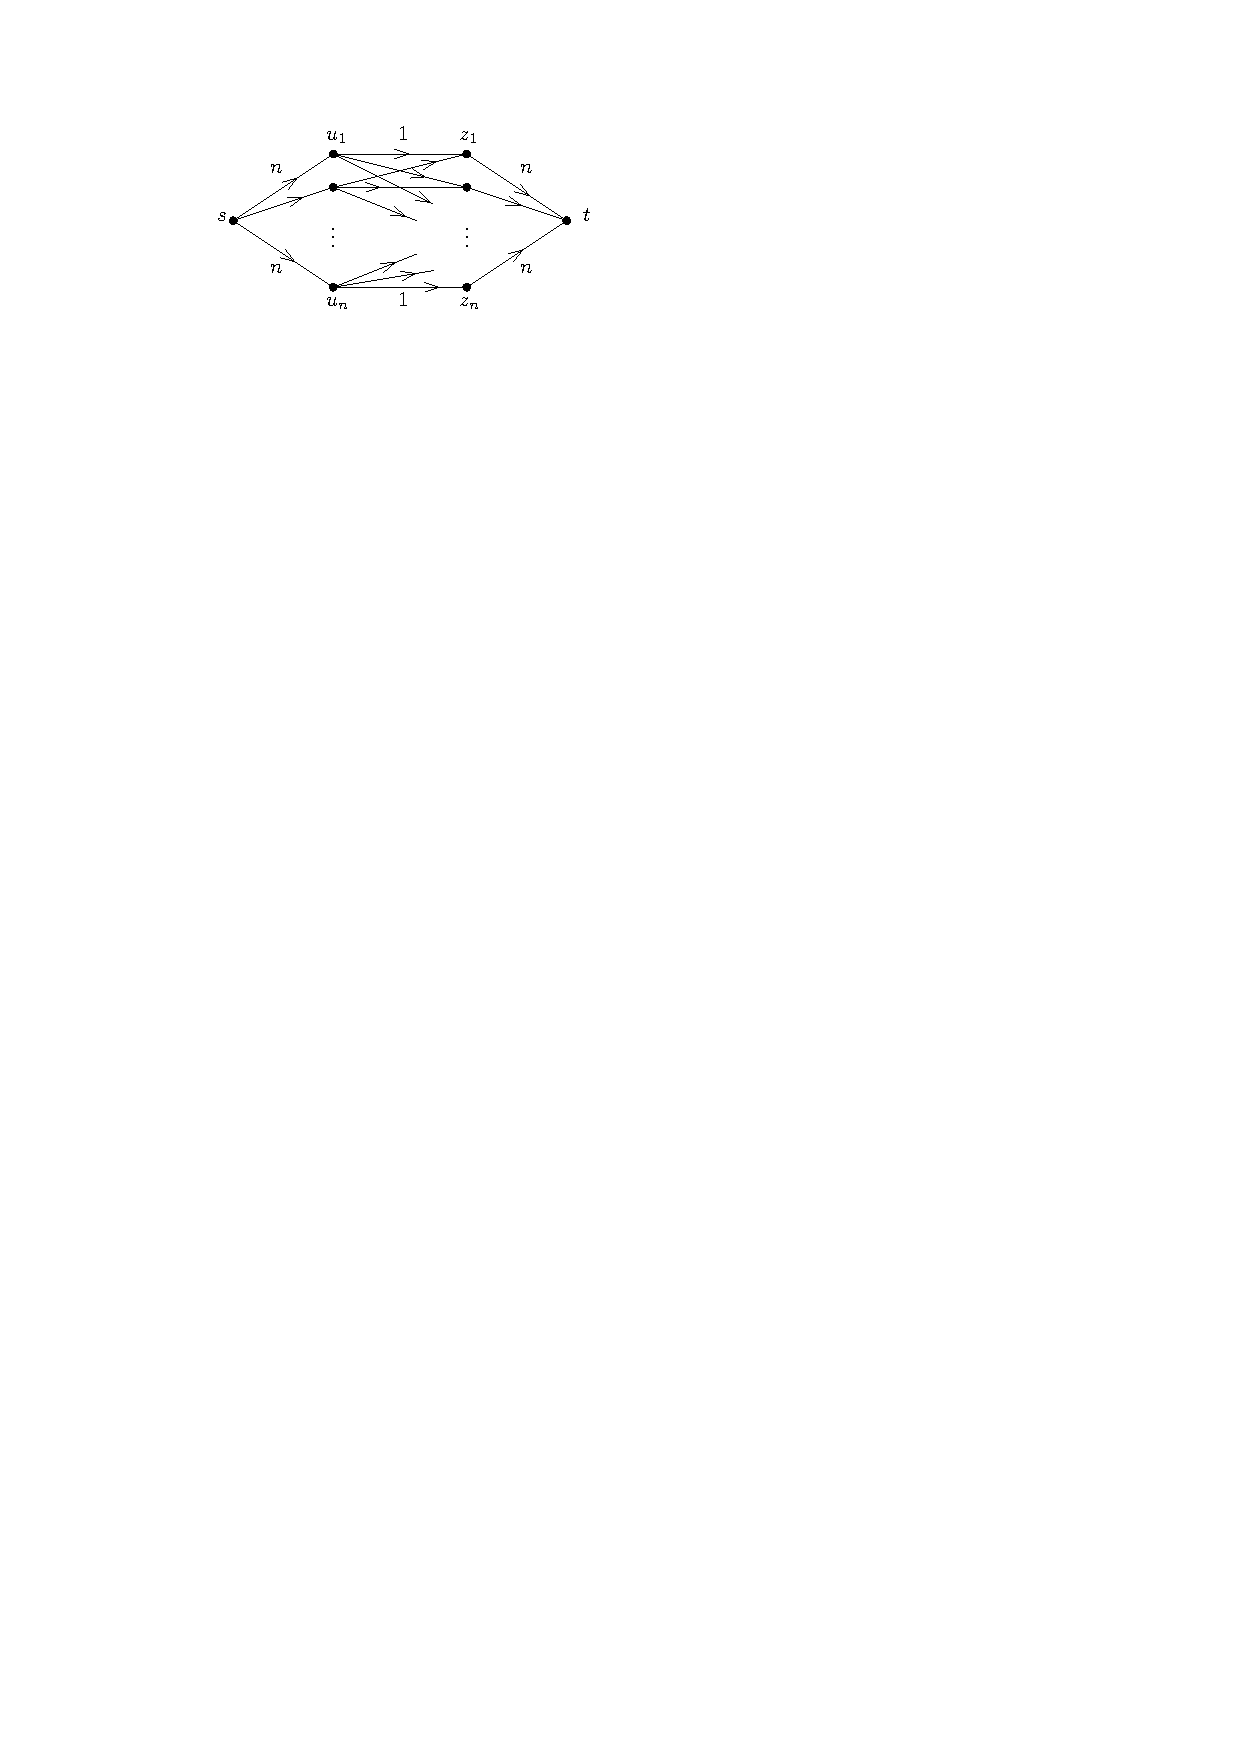
\includegraphics[scale=1]{img/relaxation-ratio-unbounded}
\caption{Graph used in the proof of \cref{thm_relaxation_ratio_unbounded}}
\label{fig_relaxation_ratio_unbounded}
\end{figure}
\begin{proof}[Proof of \cref{thm_relaxation_ratio_unbounded} using \cref{thm_mindegree_diameter_erdos}]
Let $G$ be the graph sketched in \cref{fig_relaxation_ratio_unbounded}. Formally,  let $U := \fromto{u_1}{u_n}$ and $W := \fromto{w_1}{w_n}$. For each $i$, there is an edge $(s,v_i)$ and  an edge $(w_i, t)$ with lifetime $n$ and for all $i, j$ there is an edge $(u_i, w_j)$ with lifetime 1. It is easy to see, that the optimal solution for the Menger problem for this instance is exactly $n^2$.
 First, we describe a schedule of value $\lfloor \sqrt{n} \rfloor^3$: Let $k := \lfloor \sqrt{n} \rfloor$ and consider for $i \in \fromto{1}{k}$ the sets $U_i := \fromto{u_{(i-1)k+1}}{u_{ik}}$ and $W_i := \fromto{w_{(i-1)k+1}}{w_{ik}}$. Then consider the schedule consisting out of $k$ phases, where in the $i$-th phase, we activate all edges between $s$ and $U_i$ and all edges between $W_i$ and $t$ at the beginning of the phase, and all $k^2$ edges between $U_i$ and $W_i$ in order during the phase. It is easy to see that this describes a valid schedule of value $k^3$.
 
We now claim that $\optDirStAct(I) \leq 16n^{1.5}$. If we can show this, we are done. So assume there exists a schedule $\sigma$ of value greater than $T := 16n^{1.5}$. Then, for each $k \in \fromto{1}{T}$, there is at least one path $P_{k}$ from $s$ to $t$ in $G^\sigma_{k}$. Let $(u_{i(k)}, w_{j(k)})$ be the unique edge on $P_k$ which connects $U$ and $W$ and $e_{k} := \{u_{i(k)}, w_{j(k)}\}$ be the corresponding undirected edge. For $k \neq k'$ we have $e_{k} \neq e_{k'}$. Consider the undirected graph $H'$ on vertex set $U \cup W$ and edge set $\fromto{e_1}{e_T}$. 
%Then $H'$ has average degree $2E(H') / V(H') \geq T/n$. 
We claim there is a subgraph $H$ of $H'$ which is connected and has minimum degree at least $T/(2n)$. Indeed, note that $H'$ has the property that $|E(H')| \geq T/(2n)|V(H')|$ and deleting vertices of degree less than $T/(2n)$ does not change this property. Hence we can delete those vertices until we arrive at a graph with minimum degree at least $T/(2n)$ and $H$ can be chosen as any connected component of this graph. Now, \cref{thm_mindegree_diameter_erdos} applied to $H$ yields
\begin{equation}
\radius(H) \leq 2n\frac{|V(H)| - 2}{T} + 12  \leq \frac 1{8}|V(H)|n^{-0.5}+12. \label{eq_radius}
\end{equation}
For $u_i \in U$, define $\sigma(u_i) := \sigma(su_i)$ and for $w_j \in W$, define $\sigma(w_j) := \sigma(w_jt)$. Now, a crucial observation is that by the definition of $e_k$, for each $k$ we have that both $su_{i(k)}, w_{j(k)}t \in E(G_k^\sigma)$, and therefore $|\sigma(u_{i(k)}) - \sigma(w_{j(k)})| \leq n - 1$. Define \[ L := \max_{v \in V(H)}\set{ \sigma(v) + n } - \min_{u \in V(H)} \set{\sigma(v)}, \] i.e.\ $L$ describes the maximal amount of time, such that $P_k$ contains some vertex of $V(H)$. Let $R := 1/8|V(H)|n^{-0.5} +12$. By \cref{eq_radius} and the previous observation, and by $|V(H)| \geq \delta(H) \geq 8n^{0.5}$, we have 
\begin{align*}
L &\leq 2R(n-1) + n < (2R + 1)n = 1/4|V(H)|n^{0.5} + 25n\\ 
&\leq 1/4|V(H)|n^{0.5} + 25/8|V(H)|n^{0.5} < 4|V(H)|n^{0.5}.
\end{align*}
But on the other hand, $H$ has only edges of the form $e_k$, and by definition of $L$ and $e_k$ we must have $L \geq |E(H)| \geq |V(H)|\delta(H)/2 \geq 4|V(H)|n^{0.5}$. This is a contradiction.
\end{proof} 
(Note: A more careful calculation in the previous proof yields $\optDirStAct(I) \leq 6\sqrt{6}n^{1.5}$.)

\begin{corollary}
There is a directed graph on $2n+2$ vertices such that $\optDirSTP = n^2$, but $\optDirAct = \theta(n^{1.5})$.
\end{corollary}
\begin{proof}
Let $G$ be the same directed graph like in \cref{thm_relaxation_ratio_unbounded} with additional edges $(t, u_i)$ and $(t, w_i)$ for all $i$, each having lifetime $\infty$. Then finding a spanning branching in $G$ is equivalent to finding an $s$-$t$-path in the original graph, hence the claim follows by \cref{thm_relaxation_ratio_unbounded}.
\end{proof}

Unfortunately, the idea for the proof of \cref{thm_relaxation_ratio_unbounded} can not be adapted to the case of undirected graph. Let (for even $n$) $G$ be the graph depicted in \cref{fig_relaxation_ratio_unbounded}, but without edge directions, i.e.\ we have $U = \fromto{u_1}{u_n}$, $W := \fromto{w_1}{w_n}$ and undirected edges $su_i$ and $w_it$ of lifetime $n$ and undirected edges $u_iw_j$ of lifetime 1 for all $i, j$. Then let $H := G[\fromto{u_{n/2+1}}{u_n} \cup \fromto{w_{n/2+1}}{w_n}]$ and fix some edge-coloring of $H$ with $n/2$ colors. Then consider the schedule consisting out of $n/2$ phases, where in the $i$-th phase we activate $su_i$, $w_it$, all edges of color $i$, and all edges $u_iw_j$ and $u_jw_i$ for $j \in \fromto{n/2+1}{n}$. This schedule has value $n^2/4$. So we can achieve a ratio of at least 1/4 of the solution to the Menger problem in this particular graph.

\comment{Maybe can be proven with following idea: Use the graph in \cref{fig_undirected_relaxation_ratio} with a similar argument to the previous proof and additionally Szemeredi's regularity lemma???}

\begin{conjecture}
(i) There is a family $(I_n)$ of instances of the undirected activation problem, such that $\optAct(I_n) / \optSTP(I_n) \rightarrow \infty$. (ii) There is a family $(I_n)$ of instances of the undirected $s$-$t$-activation problem, such that $\optStAct(I_n) / \optMenger(I_n) \rightarrow \infty$.
\end{conjecture}

\section{Conclusion}

\begin{itemize}
\item Computational complexity mostly solved: Both problems remain NP-complete if either treewidth or edge weights are bounded by a constant. If both are bounded, $\act$ can be solved in linear time. But we don't know whether $\stact$ can be solved polynomially in this case (but it can, if we additianlly bound the maximal size of a solution). These results are summarized in \cref{table_complexity}.
\item Understanding approximability properties is mostly open. We showed that $\act$ can not be approximated by a factor better than $7/6$. But we don't know whether an analogous result holds for $\stact$. We also were not able to find approximation algorithms for $\act$ or $\stact$ with $\bigO(1)$ approximation ratios. \comment{We could try to find algorithms with $\bigO(n)$ approximation ratios maybe? I haven't thought about that very much yet.}
\item Further research into this area therefore interesting.
\end{itemize}


\begin{table}
\begin{tabular}{r|rrrr}
& $T = \bigO(1) \land \tw = \bigO(1)$ & $l = \bigO(1) \land \tw = \bigO(1)$ & $l = \bigO(1)$ & $\tw = \bigO(1)$\\
\hline
$\act$ & $\bigO(n)$ & $\bigO(n)$ & NPC & strongly NPC \\
$\stact$ & $\bigO(n)$ & ? & NPC & (strongly?) NPC \\
\end{tabular}
\caption{Hardness results (? = unknown)}
\label{table_complexity}
\end{table}

\begin{table}
\begin{tabular}{r|rr}
& lower bound & upper bound \\
\hline
$\act$ & 7/6 & ?  \\
$\stact$ & ? & ? \\
\end{tabular}
\caption{Approximation results (? = unknown) \comment{This table not in final paper, only here for ourselves to see what's still open}}
\end{table}

\printbibliography


\appendix

\section{Connection to job scheduling}
\label{appendix:connection_act_job_scheduling}
A \emph{matroid} is defined ...
Problem \act\ is related to job scheduling in the following way: Let $G = (V, E)$ be a graph. The \emph{graphic matroid} of $G$ is the set system $\set{F \subseteq E \mid F \text{ is acyclic}}$. A \emph{base} in a matroid is set of maximal cardinality. Hence problem \act\ has the following generalization: Given a ground set $E$, lifetimes $l: E \rightarrow \N$, and some matroid $\mathcal{F} \subseteq 2^E$, find activation times such that for a maximal amount of time, the set of active elements comprises a base of $\mathcal{F}$. Now, if $E$ is a set of jobs with processing times $l$, and $\mathcal{F} = \set{F \subseteq E : |F| = k}$ is the uniform matroid of rank $k$, then the matroid activation problem is exactly the problem of maximizing the minimum machine load time when distributing the jobs onto $k$ machines.

\section{Possible idea relaxation ratio undirected}

\begin{figure}[htpb]
\centering
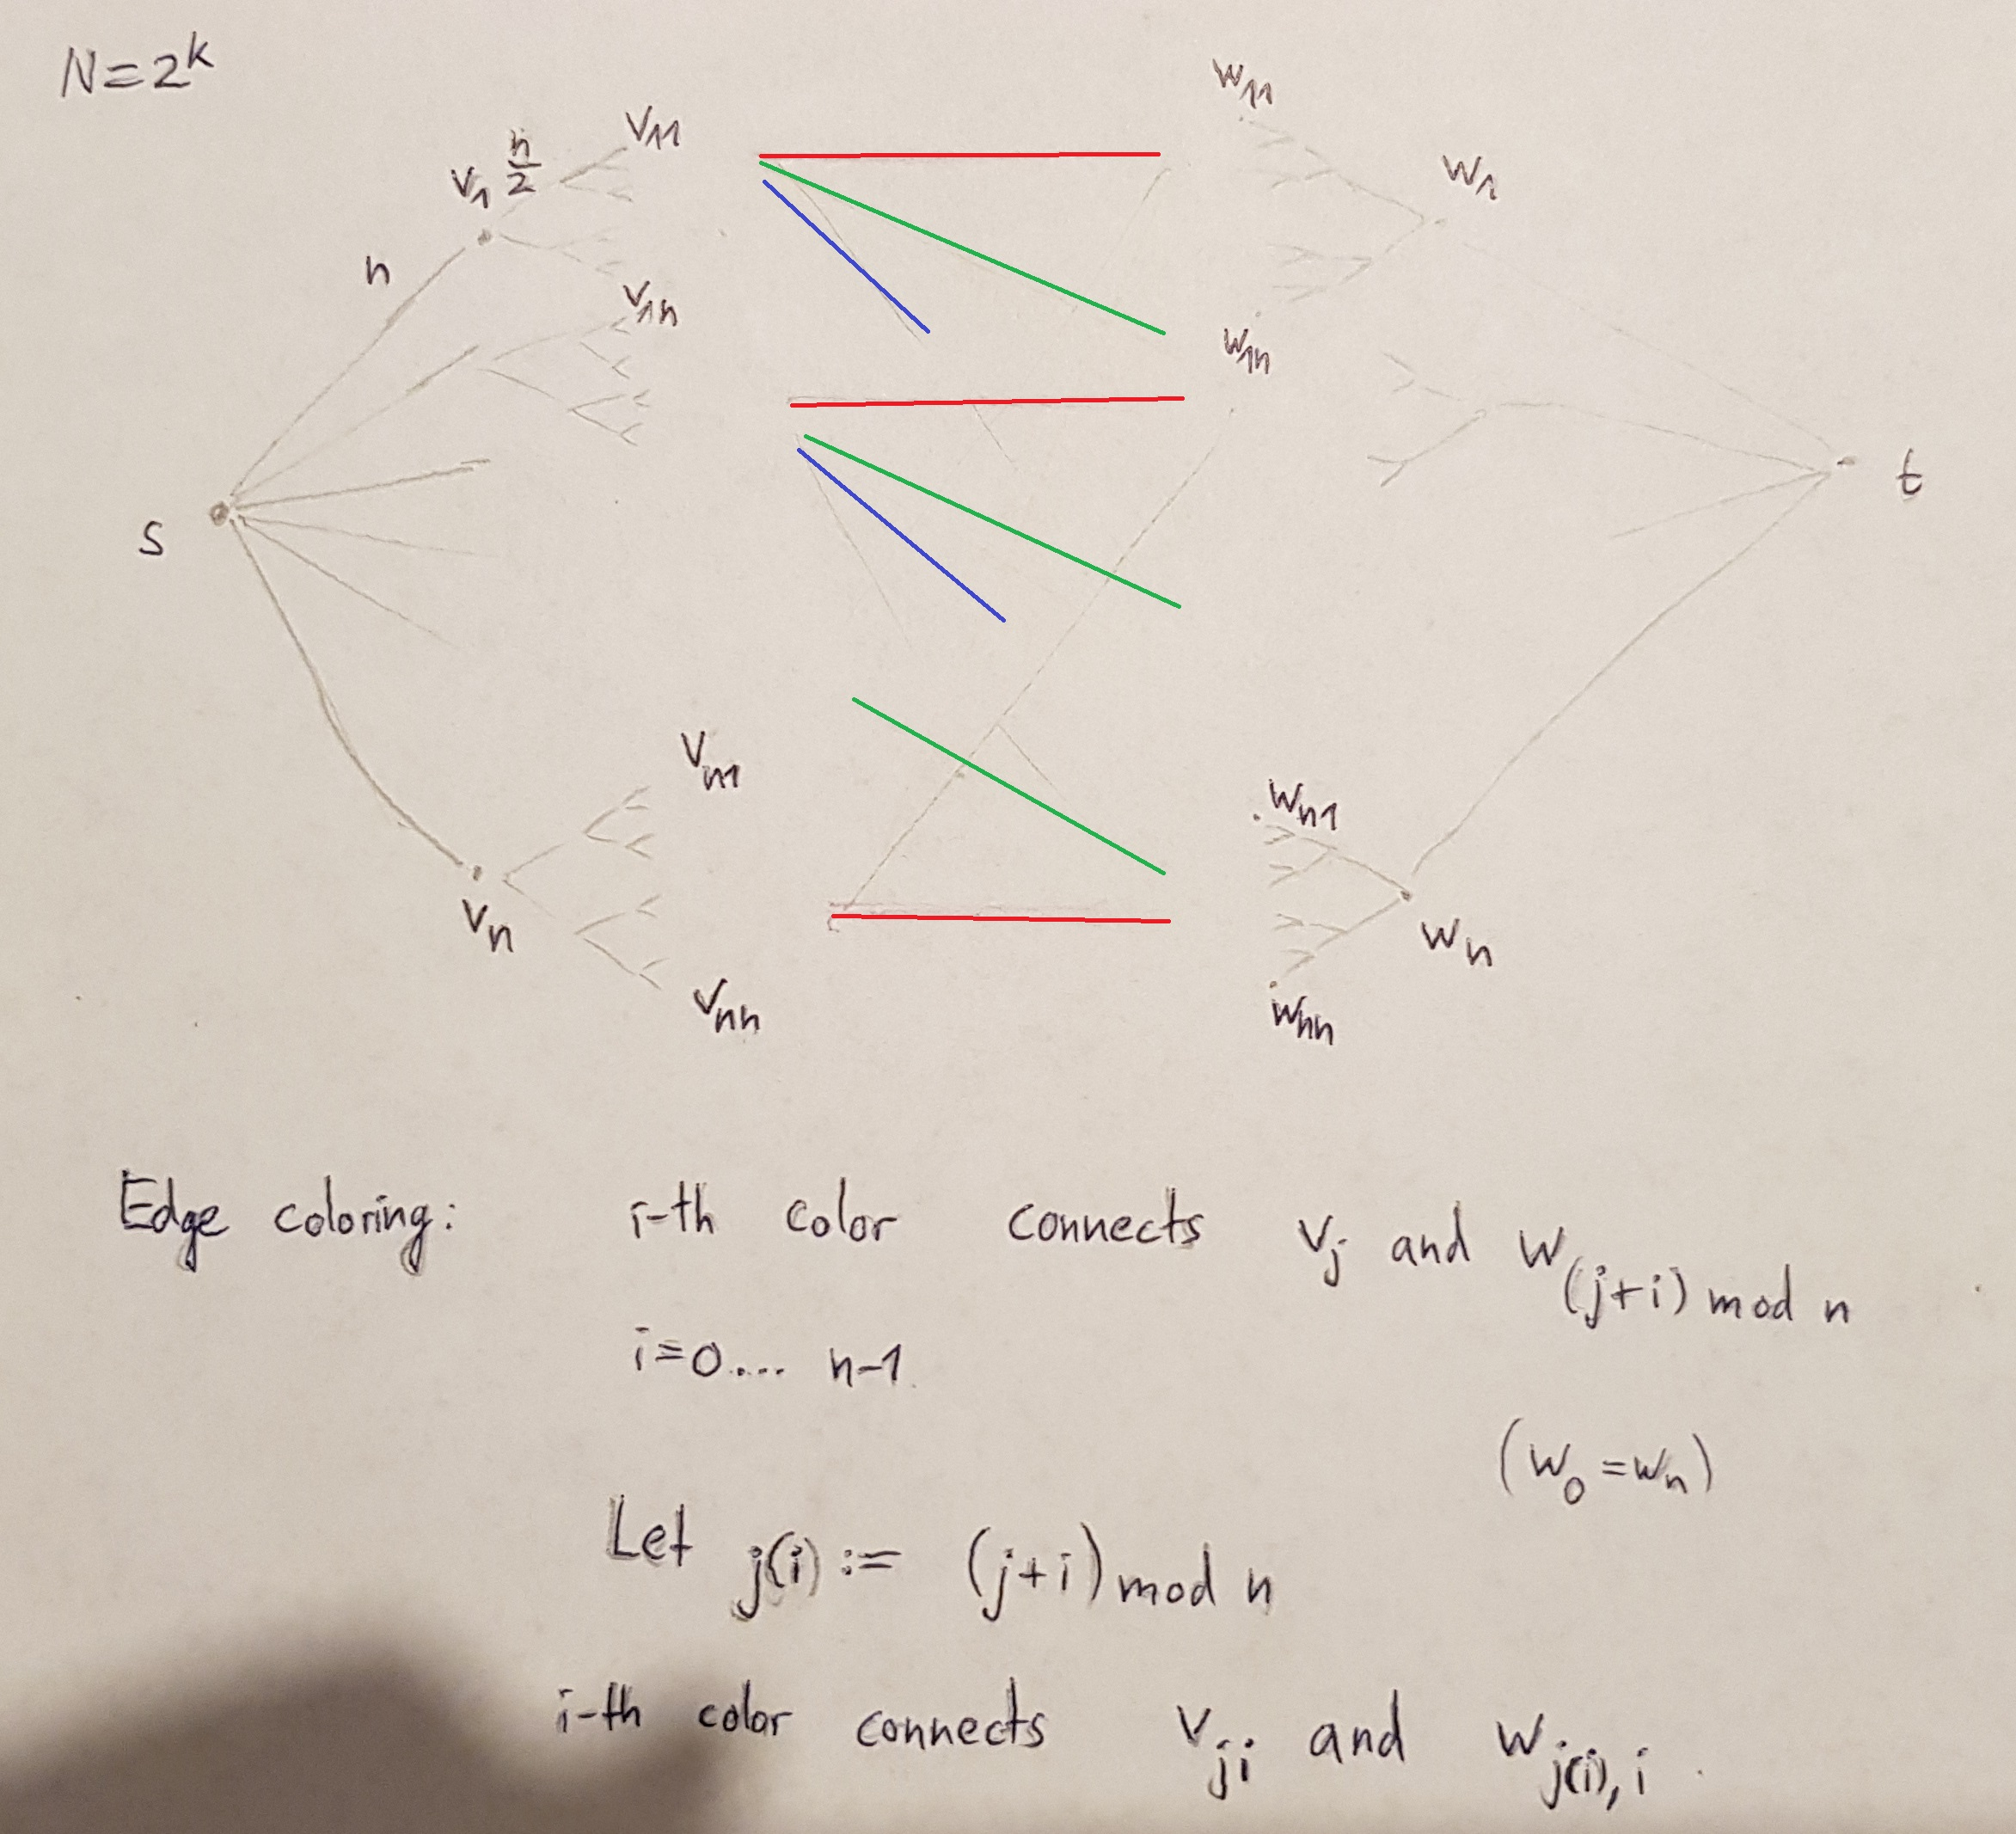
\includegraphics[width=\textwidth]{img/idea_undirected_approximation_ratio.jpg}
\caption{\comment{idea for proving an analogue of \cref{thm_relaxation_ratio_unbounded} for undirected graphs?}}
\label{fig_undirected_relaxation_ratio}
\end{figure}

\end{document}